\chapter{The e-GPU Platform}

    \section{Introduction}
    
        % Pre-introduction: The other sections are moved to the introduction chapter
        As edge computing systems continue to evolve toward greater autonomy and computational richness, the demand for accelerators capable of supporting increasingly complex and data-intensive workloads has grown substantially. This trend is particularly pronounced in emerging application domains such as real-time machine learning, biomedical signal processing, and smart sensing, where low-latency inference and high-throughput data processing are required directly on-device~\cite{co-design_vision}. These requirements have led to a gradual shift from narrowly focused fixed-function accelerators~\cite{asip, fft, cnn-accel} toward more flexible and programmable hardware solutions that can accommodate a wider range of algorithmic patterns.
    
        % Domain: GPUs
        Among the various classes of hardware accelerators designed to meet the demands of modern edge computing, graphics processing units (GPUs) have garnered interest due to their ability to offer both programmability and parallel performance within a compact and energy-aware footprint. GPUs excel at exploiting fine-grained data parallelism across multiple workloads, making them particularly effective for operations characterized by regular computational patterns and data reuse. These include machine learning inference, digital signal processing (DSP), and convolutional operations, which are increasingly central to the functionality of edge devices.
    
        % Domain: APUs
        The utility of GPUs is further enhanced when they are tightly integrated with host central processing units (CPUs) to form accelerated processing units (APUs), which enable heterogeneous computing platforms. This integration combines general-purpose software programmability with massively parallel hardware acceleration, facilitating more efficient task orchestration and minimizing data transfer latency between compute stages. As a result, APUs are well-suited for edge scenarios requiring real-time responsiveness and rapid decision-making, where compute tasks must be performed on-site with minimal energy overhead.
    
        % Problem: GPUs in TinyAI
        Despite the versatility of GPUs and their widespread use in mainstream computing platforms, their adoption in ultra-low-power edge applications (TinyAI) remains limited. This is largely due to the extreme hardware and software constraints that characterize such systems~\cite{co-design_vision}.
    
        On the hardware side, TinyAI platforms are typically battery-operated and must operate within power envelopes of only a few tens of milliwatts. Moreover, they are constrained by minimal silicon area, often limited to a few square millimeters, which places tight restrictions on compute density, memory capacity, and peripheral integration. In this context, GPU architectures must meet rigorous requirements in terms of power consumption, area efficiency, energy proportionality, and deterministic execution timing.
    
        On the software side, these platforms typically lack a full operating system, which leads to several critical limitations. In particular, the absence of a file system prohibits dynamic linking of libraries or file-based resource access, while the lack of multithreading support confines execution to a single-threaded model. These restrictions are a direct consequence of the lightweight software stacks adopted in such systems, which prioritize minimal memory usage and energy efficiency over broad functionality.
    
        The combined effect of these hardware and software constraints renders conventional GPU software stacks unsuitable for TinyAI environments. For instance, mainstream OpenCL implementations~\cite{pocl} assume the presence of system-level capabilities, such as the aforementioned file system access and multithreading, for managing kernel execution, shared memory coordination, and runtime scheduling. These features are either infeasible or too costly to implement on resource-constrained devices. Consequently, off-the-shelf GPU software frameworks cannot be directly reused in this context. Instead, lightweight software stacks must be developed from the ground up to support efficient GPU-based acceleration in this domain.
    
        % Other accelerators
        Due to these challenges, most current TinyAI systems rely on domain-specific accelerators that are carefully optimized for targeted classes of workloads. For example, coarse-grained reconfigurable arrays (CGRAs)~\cite{oe-cgra, vwr2a} provide a compromise between programmability and energy efficiency, making them suitable for irregular or control-intensive applications. Systolic arrays~\cite{cnn-accel} offer high computational density and regular data movement patterns, which are particularly beneficial for matrix and convolutional computations. Likewise, near-memory and in-memory computing (NMC/IMC) architectures~\cite{nmc, blade, maxwell} aim to reduce the energy and latency overhead associated with data transfers by co-locating computation and storage.
    
        These specialized architectures have demonstrated excellent energy efficiency and performance for their respective workload domains, significantly outperforming general-purpose CPUs in such tasks. However, they typically lack flexibility, exhibit limited software ecosystem support, and offer constrained programmability. As a result, they are less suitable for use cases involving heterogeneous or evolving workloads, rapid prototyping, or post-deployment reconfiguration. In contrast, GPUs occupy a compelling middle ground between general-purpose programmability and efficient parallel execution. They represent a promising target for broader applicability in TinyAI systems, provided their architectures and software models can be appropriately tailored.
    
        % SOTA: Commercial High-performance GPUs - Limitations
        Over the past decade, a wide range of GPU designs has been explored, spanning high-performance architectures used in desktops, servers, and data centers, as well as more energy-efficient GPUs integrated into mobile and embedded platforms. At the high end, GPUs from vendors such as NVIDIA~\cite{nvidia} and AMD~\cite{amd} feature tens of compute units and thousands of threads, supported by multi-level cache hierarchies, complex interconnects, and sophisticated software runtimes. While these designs deliver exceptional throughput and scalability for data-parallel workloads, they are unsuitable for edge deployment due to their high power consumption, extensive silicon area, and reliance on complex software infrastructure.
    
        % SOTA: Commercial Low-power GPUs - Limitations
        Embedded GPUs, such as ARM Mali~\cite{arm}, Imagination PowerVR~\cite{imagtech}, and Qualcomm Adreno~\cite{qualcomm}, address power consumption more directly by employing architectural optimizations such as clock gating, reduced memory access latency, and lightweight execution units. These designs have enabled GPU acceleration in energy-sensitive devices such as smartphones and tablets. However, they still consume hundreds of milliwatts and rely on support from full-featured operating systems like Android~\cite{android} or Linux~\cite{linux}, which remain impractical in TinyAI settings.
    
        % SOTA: Academic GPUs - Limitations
        In response to these limitations, the academic community has begun to explore lightweight GPU-like accelerators tailored to constrained systems~\cite{skybox, metasat, virgo, ventus}. These designs often reduce the number of compute units, simplify control logic, and operate within minimal system memory. Notable examples include open-source platforms like Vortex~\cite{vortex}, which implement RISC-V-compatible GPUs that support OpenCL execution on FPGAs. Other efforts propose domain-specific GPUs that attempt to strike a balance between programmability, energy efficiency, and silicon area. However, many of these solutions still rely on assumptions that do not hold in deep-constrained environments, limiting their applicability to most TinyAI devices.

        % Motivation
        In summary, while GPUs present a compelling opportunity for efficient parallel computing at the edge, their adoption in ultra-constrained systems remains underexplored. The architectural principles that make GPUs attractive, including parallelism, programmability, and performance scalability, align closely with the needs of many TinyAI workloads. Yet, harnessing these benefits within the severe constraints of ultra-low-power platforms demands a systematic rethinking of both GPU hardware and software. This challenge motivates the need to investigate how GPU architectures can be redesigned for TinyAI use cases, and how lightweight software stacks can be redeveloped to make their adoption viable. Addressing this gap has the potential to unlock new design trade-offs and capabilities for next-generation TinyAI platforms.

        % Solution: My GPU
        To deal with these limitations, this chapter introduces the embedded GPU (\mbox{e-GPU})~\cite{e-gpu}, an open-source and configurable RISC-V GPU platform for TinyAI applications. The design of \mbox{e-GPU} emphasizes modularity, allowing developers to adjust a wide range of architectural parameters, such as the number of compute units, the number of threads and warps, cache memory size, and interface bandwidth, to meet the specific power, area, and throughput requirements of their target applications. This level of tunability enables a systematic exploration of the design space and supports fine-grained trade-offs between energy efficiency and computational capability.

        % Feature: Tiny-OpenCL
        To complement the hardware platform, this chapter also introduces \mbox{Tiny-OpenCL}, a lightweight OpenCL-like software framework purpose-built for TinyAI devices. \mbox{Tiny-OpenCL} offers a simplified programming interface that mirrors the structure and semantics of conventional OpenCL, allowing developers to write parallel kernels in an intuitive way. Internally, however, it is optimized for execution environments with no operating system support, static linking of libraries, and single-threaded execution. By bridging the gap between high-level programmability and tight constraints, \mbox{Tiny-OpenCL} enables application developers to leverage the e-GPU platform without the steep learning curve and system overhead associated with traditional GPU runtimes.

        % Case study: APU
        To demonstrate the feasibility of the proposed approach, the \mbox{e-GPU} is integrated into the eXtendible Heterogeneous Energy-Efficient Platform (\mbox{X-HEEP})~\cite{x-heep}, a modular RISC-V host designed to support the exploration of custom accelerators. This integration enables the creation of a fully functional APU that supports unified memory access, lightweight interfacing, and efficient offloading of compute-intensive tasks such as machine learning and digital signal processing, all within the stringent power and area constraints of TinyAI platforms.\\\\
            
        The key contributions of this chapter are summarized as follows:

        \vspace{-1em}
        \begin{itemize}
            \item \mbox{e-GPU}~\cite{e-gpu}, an open-source and configurable RISC-V platform for exploring the feasibility and trade-offs of using GPUs in TinyAI applications.

            \item \mbox{Tiny-OpenCL}, a lightweight OpenCL implementation tailored to constrained devices to overcome the programming limitations of this application domain.
    
            \item Extensive internal configurability that enables fine-grained optimizations to match application requirements.

            \item \mbox{APU}: A full system integration of e-GPU with the \mbox{X-HEEP}~\cite{x-heep} host to demonstrate the adaptability of the proposed platform in real-world scenarios.
    
            \item A publicly released open-source repository including the complete code and documentation of \mbox{e-GPU} to support future research on TinyAI heterogeneous systems.\footnote{The complete code and documentation of the e-GPU platform are available at \url{https://github.com/esl-epfl/e-gpu}.}
        \end{itemize}
        \vspace{-1em}
        
        The remainder of this chapter is organized as follows. Section~\ref{sec:related_work} reviews relevant GPU-based platforms and highlights their limitations. Section~\ref{sec:background} provides background on GPU architecture and programming models. Section~\ref{sec:e-gpu_hardware} introduces the \mbox{e-GPU} hardware architecture, while Section~\ref{sec:e-gpu_software} describes the \mbox{Tiny-OpenCL} software stack. Section~\ref{sec:apu_system} presents the integration with the \mbox{X-HEEP} host to build the APU system. Section~\ref{sec:experimental_setup} presents the experimental setup, while Section~\ref{sec:experimental_results} the experimental results. Finally, Section~\ref{sec:conclusions} summarizes our findings.

    \section{Related Work}
    \label{sec:related_work}
    
        GPUs have emerged as high-performance accelerators for parallel workloads in domains such as machine learning and signal processing. However, their integration into TinyAI systems remains limited, primarily due to stringent constraints on power consumption, silicon area, and system-level integration.
        
        To evaluate the feasibility of GPU-based solutions in this emerging domain, it is important to review the state-of-the-art in both commercial and academic developments. Commercial GPUs, while optimized for high performance and, in some cases, energy efficiency in mobile or embedded environments, typically exceed the power budgets of TinyAI systems. In addition, these platforms often lack the transparency and configurability required for architectural exploration and domain-specific adaptation.
        
        In contrast, academic GPU platforms provide greater architectural flexibility and visibility into design trade-offs, enabling customization and exploration. However, many of these efforts are not explicitly designed to meet the ultra-low power, footprint, and programmability constraints required by TinyAI workloads.
        
        This section reviews the most relevant commercial and academic GPU efforts that inform the design of the proposed \mbox{e-GPU} platform. First, commercial architectures are analyzed in the context of their applicability to edge computing. Then, academic works are reviewed, categorizing them into software-level simulators and synthesizable hardware implementations, with an emphasis on their suitability as a foundation for GPUs tailored to TinyAI scenarios.

        \subsection{Commercial Platforms}
        
            The landscape of commercial GPUs for edge computing is populated by a range of solutions targeting the trade-off between computational performance and energy efficiency. These GPUs are typically integrated into mobile system-on-chips (SoCs) and are optimized for applications such as gaming, multimedia processing, and increasingly, on-device machine learning inference. Prominent examples include Qualcomm Adreno series~\cite{qualcomm}, ARM Mali GPUs~\cite{arm}, and Imagination Technologies PowerVR family~\cite{imagtech}.
            
            Qualcomm Adreno GPUs~\cite{qualcomm}, widely deployed in Snapdragon SoCs, offer power-efficient acceleration for compute-intensive workloads. In particular, the Adreno 600 series has been optimized for machine learning inference on mobile platforms. It employs a combination of dynamic frequency scaling and fine-grained power-gating techniques to improve energy efficiency while maintaining acceptable throughput for general-purpose and AI tasks. These features make it a popular choice in modern smartphones and edge AI products that require moderate performance in tight thermal and power envelopes.
            
            ARM Mali GPUs~\cite{arm} have evolved similarly to meet the growing demand for energy-efficient graphics and compute capabilities in embedded platforms. Architectures such as the Mali-G52 and Mali-G72 incorporate innovations such as fine-grained power gating and improved workload scheduling to reduce dynamic power consumption. These GPUs are frequently integrated into a wide variety of SoCs targeting mobile, IoT, and automotive applications, making them an important reference point when analyzing the trade-offs involved in GPU design for low-power systems.
            
            Imagination Technologies PowerVR GPUs~\cite{imagtech}, particularly the Series8XT family, further emphasize power-aware performance. Designed with tile-based rendering and energy-efficient shaders, they achieve competitive computing capabilities while maintaining a small silicon footprint. These features enable PowerVR GPUs to address performance-per-watt constraints in devices such as wearables and infotainment systems.
            
            Despite their advancements, these commercial solutions fall short of meeting the stringent constraints of TinyAI applications. Their typical power consumption ranges from hundreds of milliwatts to several watts, orders of magnitude above the tens of milliwatts budgets often required in TinyAI platforms. Furthermore, the proprietary nature of these architectures restricts access to low-level design details, preventing detailed energy characterization and architectural exploration. This opacity is a significant limitation in academic or early-stage industrial research, where full visibility and customizability are essential.
            
            As such, while commercial GPUs provide valuable insights into power-aware architectural strategies, their lack of openness and mismatch with the TinyAI power-performance envelope make them unsuitable as a basis for fully configurable or synthesizable designs targeting this emerging domain.

            \begin{table}[tp]
                \caption{Comparison of relevant academic GPU platforms based on key features.}
                \label{tbl:gpu_table}
                \centering
                \resizebox{1\textwidth}{!}{
                \begin{tabular}{|l|c|c|c|c|c|c|}
                \toprule
                \bf{GPU Platform} & \bf{Open-source} & \bf{Open ISA} & \bf{Configurable} & \bf{Synthesizable} & \bf{Integrable} & \bf{Ultra-low-power} \\
                \midrule
                GPGPU-Sim~\cite{GPGPU-sim} & \textcolor{mygreen}{\cmark} & \textcolor{myred}{\xmark} & \textcolor{mygreen}{\cmark} & \textcolor{myred}{\xmark} & \textcolor{myred}{\xmark} & \textcolor{myred}{\xmark}\\
                gem5-gpu~\cite{gem5-gpu} & \textcolor{mygreen}{\cmark} & \textcolor{myred}{\xmark} & \textcolor{mygreen}{\cmark} & \textcolor{myred}{\xmark} & \textcolor{mygreen}{\cmark} & \textcolor{myred}{\xmark}\\
                Multi2Sim~\cite{multi2sim} & \textcolor{mygreen}{\cmark} & \textcolor{myred}{\xmark} & \textcolor{mygreen}{\cmark} & \textcolor{myred}{\xmark} & \textcolor{mygreen}{\cmark} & \textcolor{myred}{\xmark}\\
                \midrule
                Skybox~\cite{skybox} & \textcolor{mygreen}{\cmark} & \textcolor{mygreen}{\cmark} & \textcolor{mygreen}{\cmark} & \textcolor{mygreen}{\cmark} & \textcolor{myred}{\xmark} & \textcolor{myred}{\xmark}\\
                ZJX-RGPU~\cite{zjx-rgpu} & \textcolor{myred}{\xmark} & \textcolor{mygreen}{\cmark} & \textcolor{myred}{\xmark} & \textcolor{mygreen}{\cmark} & \textcolor{mygreen}{\cmark} & \textcolor{mygreen}{\cmark}\\
                Vortex~\cite{vortex} & \textcolor{mygreen}{\cmark} & \textcolor{mygreen}{\cmark} & \textcolor{mygreen}{\cmark} & \textcolor{myred}{\xmark} & \textcolor{myred}{\xmark} & \textcolor{myred}{\xmark}\\
                METASAT~\cite{metasat} & \textcolor{mygreen}{\cmark} & \textcolor{mygreen}{\cmark} & \textcolor{mygreen}{\cmark} & \textcolor{myred}{\xmark} & \textcolor{mygreen}{\cmark} & \textcolor{myred}{\xmark}\\
                Virgo~\cite{virgo} & \textcolor{mygreen}{\cmark} & \textcolor{mygreen}{\cmark} & \textcolor{mygreen}{\cmark} & \textcolor{mygreen}{\cmark} & \textcolor{mygreen}{\cmark} & \textcolor{myred}{\xmark}\\
                Ventus~\cite{ventus} & \textcolor{mygreen}{\cmark} & \textcolor{mygreen}{\cmark} & \textcolor{mygreen}{\cmark} & \textcolor{mygreen}{\cmark} & \textcolor{myred}{\xmark} & \textcolor{myred}{\xmark}\\
                \midrule
                \textbf{Proposed e-GPU} & \textcolor{mygreen}{\cmark} & \textcolor{mygreen}{\cmark} & \textcolor{mygreen}{\cmark} & \textcolor{mygreen}{\cmark} & \textcolor{mygreen}{\cmark} & \textcolor{mygreen}{\cmark}\\
                \bottomrule
                \end{tabular}
                }
            \end{table}

        \subsection{Academic Platforms}
        
            While commercial GPUs are typically optimized for mainstream mobile or embedded scenarios and lack openness, the academic community has made significant efforts to explore programmable and configurable GPU architectures tailored to various computing domains. These research initiatives aim to provide open platforms that enable architectural innovation, performance evaluation, and software-hardware co-design in contexts where transparency, adaptability, and efficiency are critical.
            
            A key objective in academic research is to expose the internal design of GPUs through open-source implementations, often using open instruction set architectures (ISAs) such as RISC-V. This enables researchers to modify and extend core functionalities, introduce custom instructions, and analyze fine-grained trade-offs between flexibility, area, power, and performance. These characteristics are essential for exploring domain-specific accelerators, particularly for energy-constrained applications.
            
            To assess the relevance of academic GPU platforms to TinyAI scenarios, representative solutions are compared across six essential features:
            
            \vspace{-1em}
            \begin{enumerate}
                \item \textbf{Open-source}: Full access to the hardware and software stack is necessary for transparency and academic reproducibility.
                
                \item \textbf{Open ISA}: An open ISA, such as RISC-V, allows seamless extensions for specialized instructions and enables cross-platform toolchain compatibility.
                
                \item \textbf{Configurable}: The ability to tune key architectural parameters (e.g., thread count, memory hierarchy, warp scheduling) is essential for adapting to domain-specific requirements.
                
                \item \textbf{Synthesizable}: A synthesizable register transfer level (RTL) implementation allows precise area, power, and timing evaluation through ASIC or FPGA flows.
                
                \item \textbf{Integrable}: The GPU must support integration with host CPUs, enabling realistic CPU-GPU interactions, memory sharing, and task offloading.
                
                \item \textbf{Ultra-low-power}: The architecture should be adaptable to operation under tight power constraints (tens of milliwatts), typical of TinyAI devices.
            \end{enumerate}
            \vspace{-1em}
            
            These criteria are summarized in Table~\ref{tbl:gpu_table} and guide our analysis of prior work. The platforms span two broad categories: \emph{software simulators}, which provide rapid architectural prototyping but limited synthesis capabilities, and \emph{hardware implementations}, which expose synthesizable RTL for more accurate evaluation and integration. Each category offers distinct trade-offs in terms of realism, accuracy, and implementation complexity, and understanding these is essential for designing a GPU suitable for this domain.

            \subsubsection*{Software Simulators} 
            
                Software simulators have long been a cornerstone of academic research in GPU architecture due to their flexibility, ease of modification, and suitability for rapid prototyping. These tools provide a high-level abstraction of GPU hardware, allowing researchers to evaluate instruction throughput, memory hierarchy behavior, and scheduling strategies without the need for physical synthesis or fabrication. As a result, they are widely used in early-stage exploration of architectural ideas and workload analysis.
                
                One of the most well-established simulators is GPGPU-Sim~\cite{GPGPU-sim}, which models NVIDIA CUDA-enabled GPU architectures, particularly from the Fermi and GT200 families. It supports the execution of CUDA applications and enables detailed profiling of kernel execution at the warp and thread level. Its modular design allows extensions, making it useful for studying compute unit behavior, warp scheduling, and memory coalescing strategies.
                
                Another prominent framework is gem5-gpu~\cite{gem5-gpu}, which builds on the gem5 simulator~\cite{gem5}, a widely adopted architectural simulator for general-purpose CPUs and system-level modeling. gem5-gpu integrates GPU execution models with x86 CPU and memory system models, enabling detailed studies of CPU-GPU interactions, shared memory access latencies, and coherence strategies. This makes it particularly suitable for research on heterogeneous computing platforms with shared address spaces.
                
                Multi2Sim~\cite{multi2sim} is another GPU-capable simulation framework that models the AMD Evergreen GPU family alongside multi-threaded x86 cores. It supports OpenCL workloads and provides instruction-level execution traces for both CPU and GPU components, allowing researchers to examine parallelism, pipeline utilization, and execution bottlenecks in hybrid workloads.
                
                Despite their usefulness in architectural research, these software simulators exhibit fundamental limitations that reduce their applicability to TinyAI design exploration. Firstly, none of the platforms offer synthesizable RTL code, which is essential for accurately estimating power, area, and energy metrics —critical parameters in ultra-low-power design. Secondly, these simulators typically model proprietary GPU ISAs such as CUDA or AMD graphics core next (GCN), which restricts opportunities for customization, extension, or integration into open RISC-V-based ecosystems. Lastly, their design focus lies in modeling high-performance, desktop- or server-class GPUs, rather than the lightweight, resource-constrained architectures suitable for edge applications.
                
                As a result, while software simulators are valuable tools for early-stage functional and performance analysis, they fall short in supporting the full-stack design, optimization, and validation processes required for TinyAI platforms. In particular, their lack of synthesizability makes them unsuitable for evaluating the trade-offs required to meet stringent power budgets and area targets.

            \subsubsection*{Hardware Implementations} 
            
                Several academic GPU projects have moved beyond pure simulation and introduced synthesizable RTL implementations. These platforms enable researchers to evaluate not only architectural and functional behaviors, but also physical design metrics such as area, leakage power, and dynamic energy, factors that are essential in TinyAI systems. In this context, where tight constraints on power and silicon area dictate the feasibility of deployment, such implementations offer critical insights.
                
                One of the academic efforts in this direction is Skybox~\cite{skybox}, a RISC-V-based GPU platform developed for graphics research. Skybox supports the Vulkan API and includes a programmable rendering pipeline, making it suitable for exploring real-time graphics and shader programmability. Its architecture is designed to be modular and extensible, allowing researchers to study various aspects of rasterization and GPU scheduling. However, its reliance on PCIe-based communication with a host PC assumes a desktop-class setup. This interface model is incompatible with the memory-mapped interconnects typically used in SoC environments, especially those targeting this application domain. As a result, despite its openness and flexibility for graphics research, Skybox is poorly suited for deeply constrained systems requiring tight integration and low power.
                
                A more embedded-oriented example is ZJX-RGPU~\cite{zjx-rgpu}, which integrates an RISC-V CPU core with a custom fragment engine for graphics acceleration. Fabricated in a \SI{65}{\nano\meter} process, the platform operates at \SI{200}{\mega\hertz} and consumes around \SI{20}{\milli\watt}, occupying \SI{12.25}{\milli\meter\squared} of silicon area. These characteristics make it more compatible with the power and area budgets of TinyAI-class systems. However, its utility for academic research is limited by its closed-source nature and sparse documentation. The lack of publicly available RTL code and detailed design documentation hinders reproducibility, restricts architectural exploration, and complicates integration with open research frameworks.
                
                In contrast, Vortex~\cite{vortex} represents a significant step forward in academic GPU research. Built around the RISC-V ISA, it is designed as a general-purpose GPU (GPGPU) supporting both OpenCL and OpenGL workloads. Vortex features one or more compute units composed of single instruction multiple data (SIMD) lanes, warp scheduling logic, and a local memory subsystem, closely resembling modern GPU architectures. It also includes a full software stack based on LLVM, enabling the end-to-end compilation of OpenCL kernels into hardware-executable binaries. Synthesized at \SI{300}{\mega\hertz} in a \SI{15}{\nano\meter} educational cell library, Vortex achieves a power consumption of \SI{46.8}{\milli\watt} for a single compute unit, aligning with the TinyAI power range.
                
                However, despite its configurability and software completeness, Vortex is not natively synthesizable without significant modifications. Some of its components are simulation-only or require a redesign for back-end compatibility. Moreover, the platform is built for PC-class environments and assumes PCIe or other high-bandwidth host interfaces, making integration with lightweight SoC interconnects impractical. Its memory architecture and host expectations do not align with the constraints of this domain, which often lack an operating system, file-system access, and multithreading support. These limitations restrict its direct use in TinyAI deployments, though it remains a valuable foundation for academic GPU design.
                
                Building upon Vortex, METASAT~\cite{metasat} tailors the GPU for safety-critical aerospace systems. It integrates the Vortex core with the NOEL-V processor and the SPARROW SIMD accelerator into a heterogeneous RISC-V SoC. The platform operates under the real-time executive for multiprocessor systems (RTEMS) and the XtratuM real-time hypervisor, supporting partitioned execution for fault isolation and deterministic behavior, which are key requirements in space-grade systems. To meet the needs of real-time environments, METASAT removes OpenCL dependencies and replaces them with a statically linked execution model that is more compatible with certified software stacks.
                
                While METASAT demonstrates the feasibility of GPU integration in dependable embedded systems, its focus lies primarily in functional isolation and robustness rather than power and area optimization. The GPU component retains the complexity of Vortex, and no evaluations of low-power or tapeout design are reported. Moreover, the strong coupling with aerospace-specific toolchains and execution models limits its reusability in broader TinyAI contexts, where simplicity, energy efficiency, and configurability are the driving concerns.
                
                Another evolution based on Vortex is Virgo~\cite{virgo}, which introduces a disaggregated GPU design aimed at improving energy efficiency and scalability. Virgo clusters compute elements into matrix-level execution units, allowing more effective data reuse during matrix operations, particularly for general matrix multiplication (GEMM) kernels that dominate many deep learning workloads. The design also supports coordinated scheduling across clusters, optimizing throughput, and reducing off-chip memory accesses. Unlike many academic designs, Virgo is fully open-source, offering its RTL, runtime, and compiler stack for reproducible research.
                
                Despite its architectural strengths and energy-aware design, the scope of Virgo is toward datacenter-class inference or training applications, where workloads are large and highly structured. In contrast, TinyAI systems typically deal with irregular, smaller data sets and operate under tight memory and power constraints. Its multi-level memory hierarchy and complex interconnect scheme, while justified for large-scale parallelism, make it difficult to map onto ultra-constrained devices.
                
                The most advanced among recent academic efforts is Ventus~\cite{ventus}, which leverages the RISC-V Vector Extension (RVV) to build a high-performance single instruction multiple threads (SIMT)-capable GPGPU. Ventus introduces custom instructions for predicated execution, tensor operations, and warp synchronization, and is designed to scale up to 16 compute units and 256 warps. The platform shows significant performance improvements over Vortex, including up to \SI{87.4}{\percent} cycles per instruction (CPI) reduction and \SI{83.9}{\percent} instruction count reduction, demonstrating effective exploitation of vector and thread-level parallelism.
                
                Ventus is synthesizable and has been implemented on large FPGAs. However, the platform lacks low-power design considerations and has not been optimized for integration into embedded SoCs. Its software stack assumes the presence of an operating system and resource management on the host side, and its memory system is designed for high-throughput operation with wide buses and multiple access ports, features that incur overhead incompatible with the constraints of TinyAI systems. As such, Ventus is best viewed as a high-performance GPGPU research platform rather than a candidate for ultra-low-power acceleration.
                
                In summary, while these academic GPU platforms offer valuable insights into GPU architecture, programmability, and performance scaling, they fall short in addressing the specific needs of TinyAI devices. Most are either too power-hungry, lack SoC integration support, or require software environments that are incompatible with bare-metal execution. These limitations highlight the need for an innovative GPU solution that is fully open-source, highly configurable, synthesizable, and tailored to the power, area, and programmability constraints of the TinyAI landscape, motivating the development of the proposed \mbox{e-GPU} platform.

    \section{Background}
    \label{sec:background}
        
        To facilitate understanding of the architecture and programming model adopted by the proposed \mbox{e-GPU} platform, this section provides a concise but comprehensive overview of the relevant terminology derived from the OpenCL standard. While OpenCL is traditionally used in more powerful computing environments, its abstraction models remain highly relevant for lightweight GPU platforms targeting TinyAI, as they offer a standardized framework for parallel computation, memory organization, and execution control.
        
        The terminology is structured around four conceptual models derived from the OpenCL specification: the \emph{platform model}, the \emph{execution model}, the \emph{runtime model}, and the \emph{memory model}. Each of these models describes a distinct aspect of GPU operations and serves as a foundation for understanding how the proposed \mbox{e-GPU} executes kernels in a parallel and resource-constrained environment:

        \vspace{-1em}
        \begin{itemize}
            \item \textbf{Platform model}: It establishes the hierarchical relationship between the host CPU and one or more compute devices, such as GPUs or specialized accelerators. It defines how compute devices are organized into compute units and processing elements.
            
            \item \textbf{Execution model}: It outlines how parallel workloads are decomposed into smaller units, i.e., work-items and work-groups, and how these are mapped to the hardware. It specifies how the host launches kernels and their distribution across the available compute resources.
            
            \item \textbf{Runtime model}: It describes how kernel execution is managed at the hardware level. This includes thread instantiation, scheduling policies, synchronization mechanisms (such as barriers), and memory access coordination between threads.
        
            \item \textbf{Memory model}: It defines how data is stored, accessed, and shared between different memory regions during execution. It encompasses the organization of global, local, private, and constant memory spaces, each with distinct latency and visibility properties.
        \end{itemize}
        \vspace{-1em}
        
        Together, these four models form the conceptual backbone for describing and reasoning about GPU-based execution, both in traditional high-performance systems and in emerging ultra-low-power accelerators like the proposed \mbox{e-GPU}. The following subsections present each model in detail.

        \vspace{-1em}
        \subsection{Platform Model}
        
            The platform model, represented in Figure~\ref{fig:platform_model}, defines the high-level relationship between the host and the compute devices responsible for executing parallel workloads. In the OpenCL abstraction, the \emph{host} refers to the primary control unit of the system, typically a general-purpose CPU, that manages application logic, orchestrates memory allocation, and dispatches kernels to one or more compute devices. The host also performs runtime scheduling, memory transfers, and synchronization tasks, ensuring coherent interaction between the CPU and the compute devices.

            \begin{figure} [t]
                \centering
                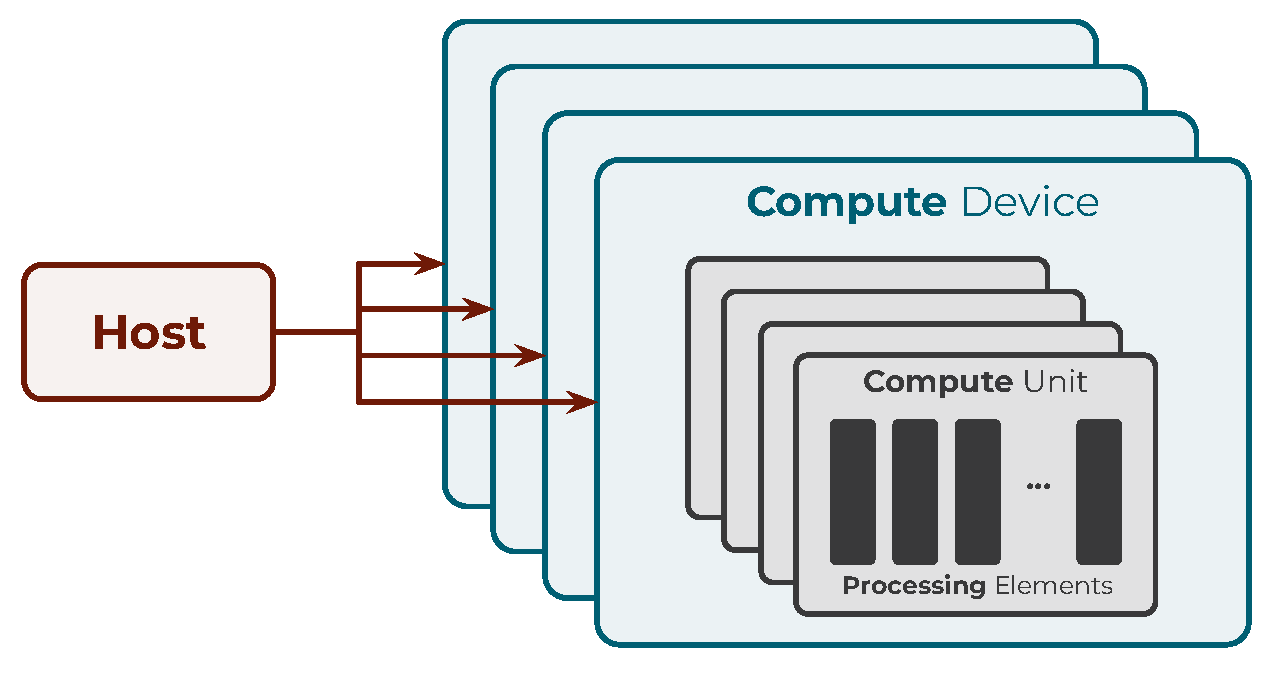
\includegraphics[width=0.9\textwidth]{./figures_e-gpu/platform_model.pdf}
                \caption{Block diagram of the OpenCL platform model.}
                \label{fig:platform_model}
            \end{figure}
            
            A \emph{compute device}, in this context, is any programmable accelerator capable of executing OpenCL kernels. These include GPUs, DSPs, or other specialized hardware blocks. The \mbox{e-GPU} can be considered one such device. Each compute device is composed of one or more \emph{compute units}, which serve as the fundamental execution blocks within the device. Compute units are responsible for executing work-groups, i.e., groups of parallel threads, and contain local resources such as thread control logic, instruction buffers, and shared data memory.
            
            Within each compute unit, there exists a set of \emph{processing elements}, which are the lowest-level functional units tasked with executing arithmetic and logic operations for individual threads, or work items. This hierarchical structure, i.e., host, compute device, compute unit, processing element, enables a clear separation between control flow and data-parallel execution. It also provides scalability, as the number of compute units and processing elements can be adjusted to match the performance and power requirements of the target application.
            
            In TinyAI systems, this platform model must be adapted to support lightweight communication protocols, minimal runtime overhead, and efficient coupling between the host and the accelerator, which is a set of constraints directly addressed in the architecture of the proposed \mbox{e-GPU}.

        \subsection{Execution Model}
    
            The execution model, represented in Figure~\ref{fig:execution_model}, describes how parallel computation is structured and mapped onto the hardware resources of the compute device. It governs the decomposition of the computational workload into manageable and concurrent tasks and specifies the mechanism by which these tasks are dispatched, scheduled, and synchronized across compute units.

            \begin{figure} [t]
                \centering
                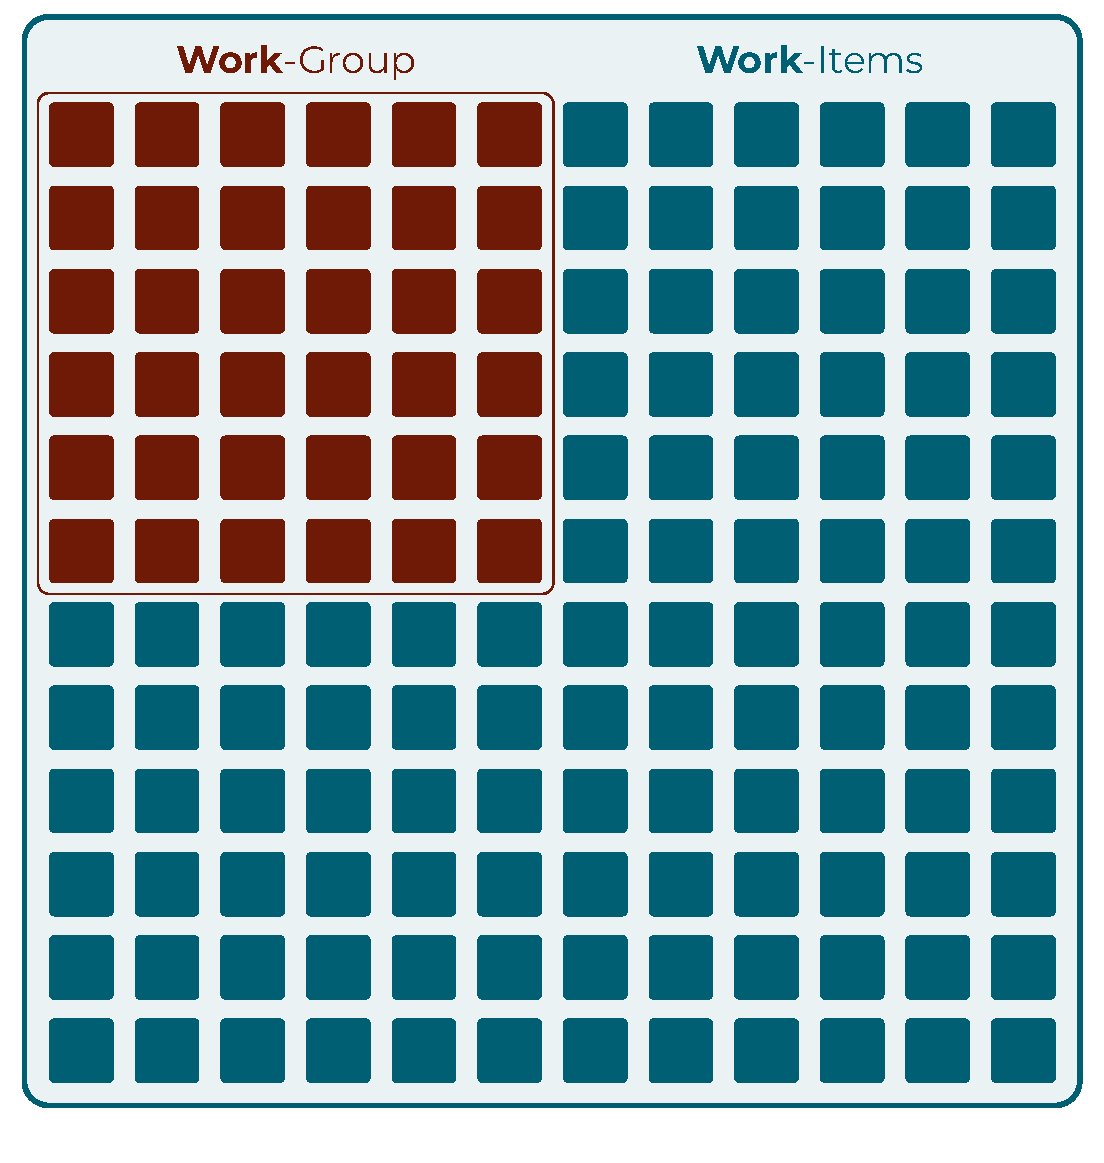
\includegraphics[width=0.55\textwidth]{./figures_e-gpu/execution_model.pdf}
                \caption{Block diagram of the OpenCL execution model.}
                \label{fig:execution_model}
            \end{figure}
    
            In the OpenCL programming model, the execution process begins on the host side. The host program issues commands to one or more compute devices, including memory allocation, kernel launching, and data transfers. A \emph{kernel} in OpenCL is a user-defined function written in a C-like language, which encapsulates the code to be executed on the compute device. When a kernel is launched, it is instantiated multiple times in parallel, once for each work-item, to operate on different segments of the input data.
    
            A \emph{work-item} represents a single thread of execution and is associated with a unique \emph{global ID}, which determines the portion of data it will process. Work-items are organized into \emph{work-groups}, each of which is assigned to a single compute unit on the target device. This two-level hierarchy, work-items within work-groups, facilitates both fine-grained data parallelism and efficient resource sharing.\\

            \begin{figure} [t]
                \centering
                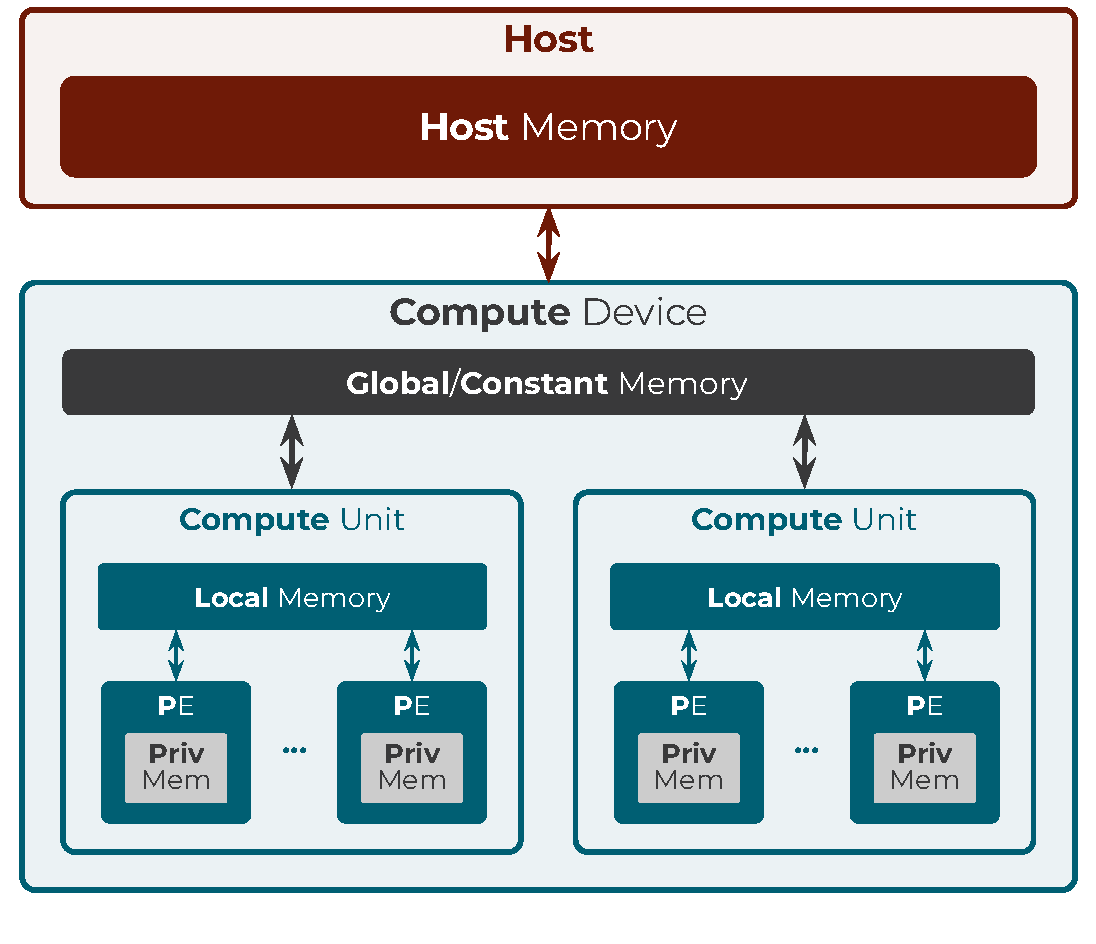
\includegraphics[width=0.7\textwidth]{./figures_e-gpu/memory_model.pdf}
                \caption{Block diagram of the OpenCL memory model.}
                \label{fig:memory_model}
            \end{figure}
    
            Within each work-group, work-items can:

            \vspace{-1em}
            \begin{itemize}
                \item Access a local memory that is private to the work-group and allows low-latency data exchange among its work-items.
                \item Coordinate execution through explicit synchronization \emph{barriers}, which ensure that all work-items in the group reach a certain point in the program before any can proceed.
            \end{itemize}
            \vspace{-1em}
    
            The number of work-items launched for a kernel is defined by the \emph{global size}, which determines the total number of kernel instances executed. The \emph{local size}, on the other hand, specifies the number of work-items per work-group. These two parameters control how work is partitioned across the compute device and have a direct impact on performance, occupancy, and memory behavior.
    
            In the context of the proposed \mbox{e-GPU}, the execution model is adapted to the constraints of TinyAI systems, where work-group sizes, synchronization scope, and memory sharing must be tightly controlled to meet strict energy and area budgets.

        % \vspace{-1em}
        \subsection{Runtime Model}
    
            The runtime model specifies how kernel execution is managed and scheduled at the hardware level. It captures the internal mechanics of how threads are instantiated, grouped, scheduled, and synchronized within a compute unit. Understanding this model is essential for evaluating the performance and resource utilization characteristics of GPU architectures, particularly in the context of resource-constrained systems.
    
            At the most granular level, a \emph{thread} represents a single instance of a kernel function being executed by a processing element. Each thread maintains its own private state, including a dedicated program counter and a private register file. In practice, hardware implementations often group threads into larger units known as \emph{warps}, which are sets of threads that execute the same instruction in lockstep. Multiple warps can be active in a compute unit concurrently, interleaving execution to hide memory latency and improve throughput.
    
            Warp-level execution introduces a trade-off: while it enables efficient SIMD-like parallelism, divergent control flow (i.e., threads taking different branches) must be serialized, potentially reducing efficiency. The proposed \mbox{e-GPU} addresses this trade-off by supporting a configurable number of active warps per compute unit and by exposing barriers for warp synchronization without requiring heavyweight runtime features.
    
        \subsection{Memory Model}
        
            The memory model, represented in Figure~\ref{fig:memory_model}, defines how different types of memory are organized and accessed by parallel threads during kernel execution. In the OpenCL specification, memory is logically divided into distinct regions, each with specific visibility, latency, and allocation behavior. These regions reflect common hardware implementations in both high-performance and TinyAI GPU architectures.

            The four primary memory regions are defined by OpenCL as follows:

            \vspace{-1em}
            \begin{itemize}
                \item \textbf{Global Memory}: The main memory accessible by all work-items across all work-groups. It typically resides in external DRAM or in a large on-chip memory shared by all compute units. Global memory accesses have the highest latency and energy cost, and minimizing such accesses is essential for energy-constrained systems like TinyAI platforms.
            
                \item \textbf{Local Memory}: Shared among all work-items in a single work-group and typically implemented as a low-latency scratchpad within the compute unit. It facilitates intra-group communication and temporarily buffers data to reduce repeated global memory accesses.
            
                \item \textbf{Private Memory}: Private to each work-item in a work-group, used to store registers and temporary variables. This region is often mapped to physical registers in the processing elements. Efficient register allocation is essential to avoid spilling into local or global memory.
            
                \item \textbf{Constant Memory}: A read-only region initialized by the host and accessible by all work-items. It is typically used to store configuration parameters, coefficients, or lookup tables that remain unchanged during kernel execution.
            \end{itemize}
            \vspace{-1em}
            
            The memory model plays a critical role in energy efficiency and must be carefully co-designed with the execution pipeline and kernel software to achieve the desired performance-power trade-offs. In the \mbox{e-GPUs}, these memory spaces are implemented using configurable structures, ranging from scratchpads to small caches.

    \section{e-GPU Hardware}
    \label{sec:e-gpu_hardware}
    
        This section presents the architecture of the proposed \mbox{e-GPU}, a lightweight and configurable graphics processing unit designed for energy-efficient parallel computing in TinyAI scenarios. The \mbox{e-GPU} is engineered to deliver sufficient computational throughput for data-parallel workloads while adhering to the strict constraints on area, power, and energy that define this domain.
        
        Unlike traditional GPUs, which are typically optimized for high-performance environments, the \mbox{e-GPU} adopts a streamlined and modular architecture. It features a minimalistic pipeline, simplified control logic, and a configurable execution model that provides just-enough parallelism without incurring the overheads of complex designs. Central to its design philosophy is a tight hardware–software co-design methodology: the architecture exposes key hardware parameters, such as thread counts, warp size, memory hierarchy configuration, and synchronization primitives, to the software stack. This transparency enables the compiler and runtime system to fine-tune kernel execution for specific deployment scenarios, enhancing both energy efficiency and resource utilization.
        
        Figure~\ref{fig:gpu_architecture} illustrates a high-level view of the \mbox{e-GPU} architecture, including its main components such as compute units, memory hierarchies, and control logic. The entire design is implemented in parameterized SystemVerilog, allowing developers to instantiate different architectural variants tailored to their specific application requirements and constraints. Table~\ref{tbl:gpu_knobs} lists the primary configuration parameters that govern these architectural knobs.
        
        The remainder of this section provides a detailed description of the \mbox{e-GPU} internal components. Each subsection highlights the key design trade-offs and co-optimization strategies employed to deliver a programmable, power-efficient accelerator compatible with the aforementioned OpenCL models.

        \begin{figure} [t]
            \centering
            
\includegraphics[width=1\textwidth]{./figures_e-gpu/e-gpu.pdf}
            \caption{High-level architecture of the proposed \mbox{e-GPU} platform, highlighting its modular components.}
            \label{fig:gpu_architecture}
        \end{figure}

        \subsection{Compute Unit}
        
            The compute unit serves as the fundamental architectural block of the \mbox{e-GPU}, responsible for executing data-parallel workloads in accordance with the OpenCL models. Each compute unit implements a lightweight and configurable RISC-V pipeline derived from the Vortex core~\cite{vortex}, which has been modified and extended to meet the strict power, area, and execution constraints of TinyAI systems.
            
            At its essence, the compute unit supports a fine-grained multithreading model in which a configurable number of warps execute concurrently within a single unit. Each warp consists of a configurable number of threads operating in lockstep under the SIMT paradigm. The degree of parallelism is statically defined at design time via SystemVerilog parameters that control both the number of concurrent warps and the number of threads per warp. Increasing the number of threads enhances data-level parallelism by scaling the number of processing elements, while increasing the number of warps improves throughput and latency hiding through warp-level interleaving.
            
            To comply with the tight area and energy budgets typical of TinyAI deployments, the compute unit omits floating-point support and is optimized for integer and fixed-point arithmetic. These operations are sufficient for many inference workloads, including lightweight convolutional neural networks (CNNs), finite impulse response (FIR) filters, and simple fast Fourier transforms (FFTs). This simplification significantly reduces the silicon footprint and avoids the high energy costs associated with floating-point units.
            
            Energy efficiency is further enhanced through a custom RISC-V instruction, \emph{Sleep\_Req}, introduced to support low-overhead kernel finalization. When issued by the final work-item of a work-group, this instruction stalls the issuing warp until all previously fetched instructions have been executed. Once all threads in the warp reach this state, the compute unit emits an event to the GPU controller, signaling task completion and eligibility for shutdown. The controller can leverage this event to trigger energy-saving mechanisms such as clock gating or power gating, thereby minimizing both static and dynamic power consumption when the compute unit is idle.

            \begin{table}[tp]
                \caption{Configurability knobs of the presented e-GPU platform.}
                \label{tbl:gpu_knobs}
                \centering
                \resizebox{0.65\textwidth}{!}{
                \begin{tabular}{|l|}
                \toprule
                \bf{Hardware}\\
                \midrule
                \textcolor{myred}{\textbullet} Number of compute units (CUs).\\
                \textcolor{mygreen}{\textbullet} Number of threads running in parallel on each CU.\\
                \textcolor{myred}{\textbullet} Number of warps running concurrently on each CU.\\
                \textcolor{mygreen}{\textbullet} Size of the instruction cache.\\
                \textcolor{myred}{\textbullet} Number of banks in the instruction cache.\\
                \textcolor{mygreen}{\textbullet} Line size of the instruction cache.\\
                \textcolor{myred}{\textbullet} Size of the data cache.\\
                \textcolor{mygreen}{\textbullet} Number of banks in the data cache.\\
                \textcolor{myred}{\textbullet} Line size of the data cache.\\
                \toprule
                \bf{Software}\\
                \midrule
                \textcolor{mygreen}{\textbullet} Base address of the kernel.\\
                \textcolor{myred}{\textbullet} Base address of the stacks.\\
                \textcolor{mygreen}{\textbullet} Size of the stacks.\\
                \bottomrule
                \end{tabular}
                }
            \end{table}
            
            In alignment with the overall modular and configurable philosophy of the \mbox{e-GPU}, the number of instantiated compute units is a tunable design parameter. Systems with stringent area or energy constraints may be configured with a single compute unit to execute kernels serially or with limited parallelism. In contrast, more demanding applications, such as real-time biomedical processing or dense convolutional workloads, can scale the number of compute units to increase parallel throughput. This architectural flexibility supports application-specific tailoring and facilitates exploration of the design space across a range of TinyAI deployment scenarios.

        \subsection{Memory Hierarchy}
        
            The memory hierarchy of the proposed \mbox{e-GPU} adopts a unified address space in which both the host main memory and the global memory visible to the \mbox{e-GPU} map to the same physical region. This design eliminates the need for explicit data transfers between separate memory domains, simplifying programmability and reducing both software complexity and memory footprint. As a result, TinyAI workloads benefit from more efficient and transparent execution.
            
            Each compute unit is equipped with a private instruction cache, while all compute units share a single data cache. The use of private instruction caches ensures that compute units do not interfere with each other when fetching instructions. This improves scalability and reduces cache miss rates, particularly when multiple kernels are executed concurrently or when divergence occurs across warps. On the data side, the shared cache facilitates reuse of common inputs and intermediate results. For example, data loaded during one kernel execution can remain cached and be reused by subsequent kernels, provided the cache capacity is sufficient. This reuse reduces redundant memory transfers and contributes to the energy efficiency required by TinyAI applications.
            
            The cache architecture builds upon the Vortex cache~\cite{vortex} and features a direct-mapped, multi-bank structure with a line-interleaved addressing scheme. This organization distributes memory lines across banks to improve throughput and minimize access contention. Support for outstanding memory requests allows subsequent warps to issue new memory accesses even when previous requests are stalled, improving pipeline utilization and hiding memory latency.
 
            Several cache parameters are configurable at design time via SystemVerilog parameters, allowing architectural tailoring to specific application needs:
            
            \vspace{-1em}
            \begin{itemize}
                \item \textbf{Cache size}: It defines the total storage capacity of the cache. A larger cache can accommodate bigger working sets, leading to higher hit rates and reduced reliance on high-latency global memory. However, it comes at the cost of increased area and power consumption.
            
                \item \textbf{Number of banks}: It specifies how many independent memory banks the cache is divided into. A higher number of banks enables greater memory access parallelism by allowing multiple threads or warps to access the cache simultaneously. However, poor access patterns may still lead to bank conflicts, limiting performance.
            
                \item \textbf{Line size}: It determines the number of bytes fetched or stored per cache access. Larger line sizes can improve bandwidth utilization for spatially localized memory accesses, but may increase latency and cache pollution for irregular or fine-grained access patterns.
            \end{itemize}
            \vspace{-1em}
            
            Each memory bank is encapsulated within a wrapper that enables integration with production-grade SRAM macros. This enables the accurate evaluation of the memory hierarchy in terms of timing, area, and power during the physical design phase.
            
            To enable parallel access across multiple warps and compute units, the data cache includes a redesigned interface that supports multithreaded memory requests. Each compute unit can issue one request per active thread in parallel and receive a unified response stream. Input and output data are selectively masked based on the requesting thread, preserving correctness while maximizing bandwidth utilization. When bank conflicts are avoided, this interface enables fully concurrent memory accesses across all active threads and warps.
            
            At the system boundary, the memory interface bridges internal memory transactions with the host bus through a three-stage process:

            \vspace{-1em}
            \begin{enumerate}
                \item \textbf{Cache miss handling}: When a cache miss occurs, the cache issues a request to retrieve an entire cache line from the host memory. To align with the memory interface granularity, the line is broken down into a sequence of 32-bit word transactions, enabling compatibility with systems that operate on word-level transfers.
            
                \item \textbf{Protocol translation}: The serialized word transactions are translated into the open bus interface (OBI) protocol~\cite{obi}, a lightweight and low-power memory-mapped interface widely adopted in embedded systems. This protocol provides efficient handshaking and address-data signaling suitable for tightly constrained environments.
            
                \item \textbf{Output arbitration}: A dedicated arbiter~\cite{bus} manages access to the shared output port that connects the \mbox{e-GPU} memory subsystem to the host bus. The arbiter ensures fair and efficient distribution of memory bandwidth among competing requests from different caches, preventing starvation and maintaining high throughput under contention.
            \end{enumerate}
            \vspace{-1em}
            
            The proposed memory hierarchy combines flexibility and energy efficiency to enable scalable execution and effective resource sharing, aligning well with the stringent constraints and performance requirements of TinyAI applications.

        \subsection{Controller}
        
            The \mbox{e-GPU} integrates a dedicated controller responsible for orchestrating kernel execution, managing the power state of compute units, and coordinating communication with the host system. This controller serves as the central control logic of the GPU and exposes a memory-mapped interface accessible by the host processor. Through a set of configuration and status registers, the host can initiate or halt kernel execution, reset the internal state of the GPU, and monitor the completion status of compute units. These registers provide a lightweight yet flexible interface for software-driven control, simplifying integration with software environments commonly used in TinyAI platforms.
            
            To enhance energy efficiency, the controller incorporates a power management unit that interfaces with the aforementioned RISC-V extensions. This unit leverages the custom \emph{Sleep\_Req} instruction, issued by each compute unit upon workload completion, to trigger local shutdown. As soon as a compute unit finishes executing its assigned kernel and issues the corresponding sleep request, the controller detects the event and deactivates the unit through clock gating or power gating, depending on hardware support. This strategy ensures that inactive compute units do not consume switching or leakage power, significantly reducing the overall energy footprint.
            
            Once all compute units have completed execution and signaled their status, the controller asserts an external interrupt to notify the host CPU. This interrupt-driven mechanism eliminates the need for polling and minimizes host-side power consumption, resulting in a highly efficient and responsive execution flow.

    \section{e-GPU Software}
    \label{sec:e-gpu_software} 
        
        This section describes the \mbox{Tiny-OpenCL} framework, a lightweight and highly optimized implementation of the OpenCL standard developed to enable kernel compilation and execution on the proposed \mbox{e-GPU} architecture. The framework is designed to bridge the gap between standardized GPU programming models and the hardware constraints of TinyAI platforms.
    
        \mbox{Tiny-OpenCL} maximizes compatibility with existing GPU software by preserving key elements of the OpenCL programming interface, including kernel semantics, memory abstractions, and host-device synchronization mechanisms. At the same time, it ensures portability and efficiency by minimizing runtime overhead and supporting integration into bare-metal environments.
    
        By enabling high-level GPU kernels to run efficiently on the \mbox{e-GPU}, \mbox{Tiny-OpenCL} serves as the software backbone of the proposed accelerator platform. It provides the necessary abstractions to program and manage the hardware, while exposing enough control to allow fine-grained optimization of memory access patterns, thread hierarchies, and kernel scheduling.
    
        The following subsections provide a detailed overview of the framework, covering both the compilation strategy and the execution flow.
    
        \subsection{Tiny-OpenCL Compilation}
        
            The \mbox{Tiny-OpenCL} compilation strategy provides the minimal software infrastructure required to compile OpenCL kernels for the proposed \mbox{e-GPU}. It bridges the gap between high-level kernel programming and the low-level execution requirements of a lightweight GPU architecture. The framework is composed of two main stages: the creation of a static kernel library and the transformation and compilation of a user-defined OpenCL kernel, as illustrated in Figure~\ref{fig:comp_flow}.
    
            The static library, \emph{kernel\_lib.a}, includes a set of software components built using the standard RISC-V GNU toolchain~\cite{riscv_toolchain}:

            \vspace{-1em}
            \begin{itemize}
                \item \textbf{SIMT RISC-V Extension API~\cite{vortex}}: It exposes low-level control over parallel execution. This includes activation and deactivation of threads and warps, divergence handling through split and join instructions, and the management of synchronization barriers.
                
                \item \textbf{Startup functions}: They initialize the system at runtime. They configure architectural parameters, set up internal control registers, and compute the base stack pointer for each thread, ensuring correct memory allocation.

                \item \textbf{Scheduling functions}: They distribute work-items across compute units and active warps. They manage dynamic scheduling decisions and enforce correct execution semantics, adapting the workload distribution to the hardware configuration selected at design time.
            \end{itemize}
            \vspace{-1em}

            After the static kernel library is created, a user-defined OpenCL kernel, \emph{kernel.cl}, is processed. An example implementing a matrix multiplication is shown in Figure~\ref{fig:code_opencl}. The kernel is processed through a custom lightweight parser that performs the necessary transformations to convert the kernel source into a C function, \emph{kernel.c}, with equivalent semantics. This translation includes the handling of kernel arguments, memory qualifiers, and thread index computations. The resulting C function is compiled and linked with the \emph{kernel\_lib.a} library to produce a standalone binary, \emph{kernel.elf}, ready to be loaded and executed by the \mbox{e-GPU}.

            \begin{figure} [t]
                \centering
                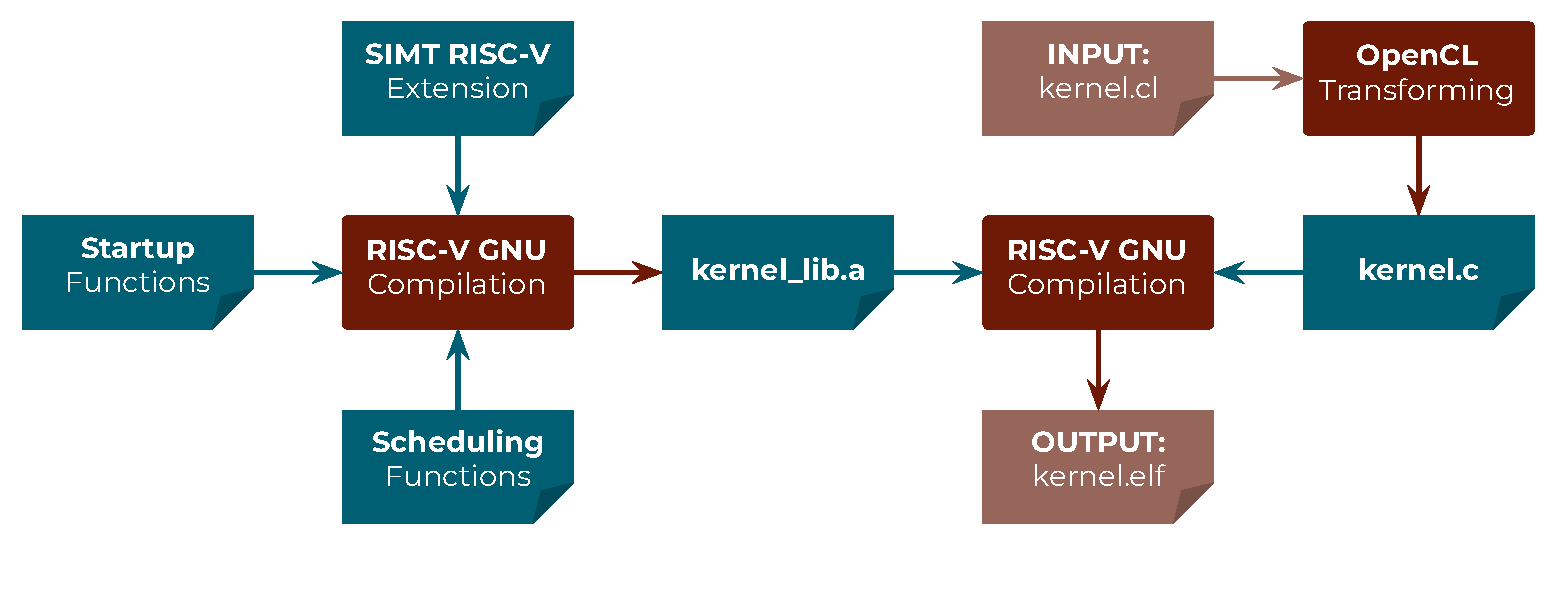
\includegraphics[width=1\textwidth]{./figures_e-gpu/tiny_opencl.pdf}
                \caption{Block diagram of the \mbox{Tiny-OpenCL} kernel compilation flow.}
                \label{fig:comp_flow}
            \end{figure}
    
            A dedicated memory region is reserved in the kernel address space for storing execution arguments provided by the host. This includes global and local sizes, input and output buffer pointers, and other application-specific parameters.
    
            To enhance configurability and portability, the framework supports several architectural and execution-time knobs, listed in Table~\ref{tbl:gpu_knobs}. Among these, the \emph{kernel base address} can be customized to allow execution from arbitrary memory offsets, while the \emph{thread stack base address and size} can be tuned to fit different workloads and memory layouts. These options enable developers to optimize the software stack for specific application domains.
    
        \subsection{Tiny-OpenCL Execution}
        
            Once the OpenCL runtime, executing on the host processor, as described in Section~\ref{sec:apu_system}, offloads a task to the \mbox{e-GPU}, kernel execution proceeds through three well-defined phases: \emph{startup}, \emph{scheduling}, and \emph{processing}. Each phase is designed to ensure that the hardware resources of the accelerator are correctly initialized, efficiently utilized, and dynamically adapted to the workload requirements, thereby maximizing performance and energy efficiency.
    
            \subsubsection*{Startup Phase}
                
                At the beginning of kernel execution, each compute unit enters a single-thread mode, in which only one warp with a single thread is active per unit. This restricted configuration allows for deterministic system setup and reduces initialization complexity. During this phase, the startup functions, compiled as part of the \emph{kernel\_lib.a} library, are executed to perform critical system configuration tasks. These include activating all parallel warps and threads that will be used during the processing phase, and computing and assigning per-thread resources such as stack pointers. Once these operations are completed, compute units return to single-thread mode and transition to the scheduling phase.
    
            \subsubsection*{Scheduling Phase}
            
                In this phase, the kernel execution context is analyzed, and parallelism is mapped onto the available hardware resources. Specifically, the scheduling functions read the \emph{global size} and \emph{local size} values from the memory-mapped kernel argument region, determining the total number of work-items to be executed and how they are organized into work-groups.
        
                Using this information, combined with architectural parameters obtained from the control and status registers (CSRs) of the \mbox{e-GPU}, such as the number of active compute units, available threads, and concurrent warps, the scheduler computes a resource allocation plan. Work-items are distributed across threads to maximize utilization of compute units and memory bandwidth. Simultaneously, unused resources are explicitly deactivated to minimize dynamic and leakage power consumption, contributing to energy efficiency.

                \begin{figure} [t]
                    \centering
                    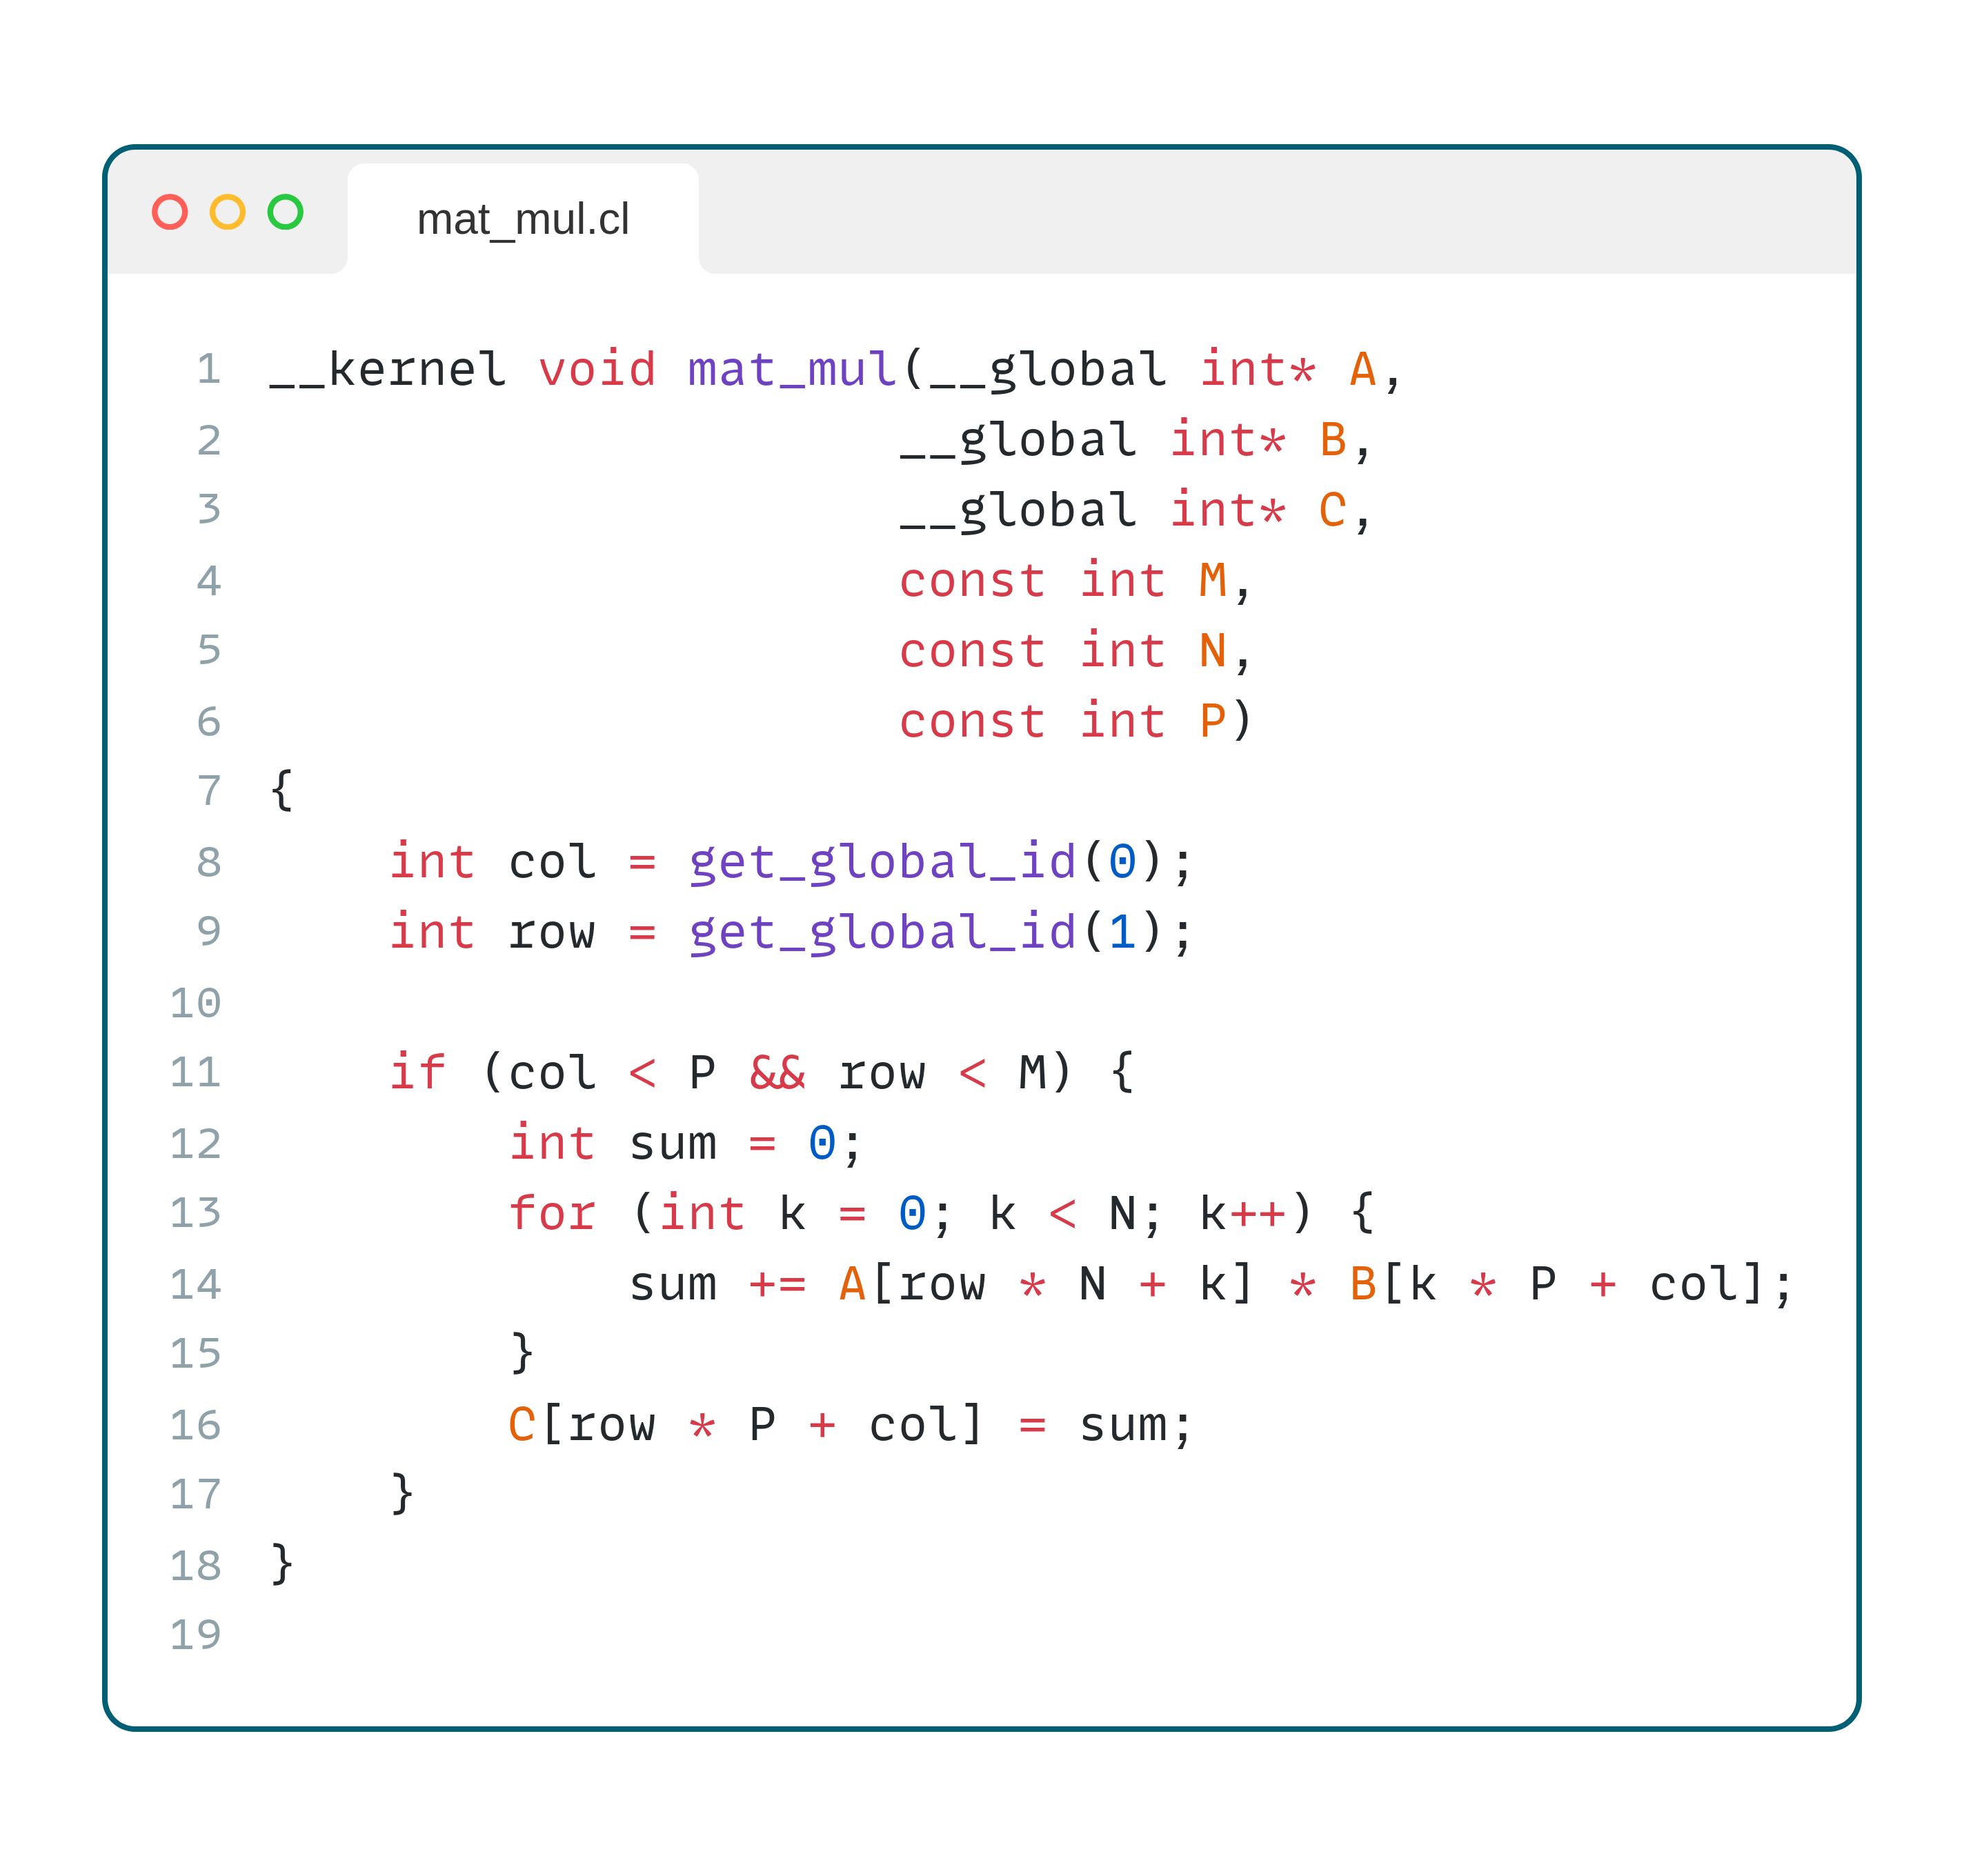
\includegraphics[width=0.85\textwidth]{./figures_e-gpu/snippet.png}
                    \caption{Code snippet of a matrix multiplication in OpenCL.}
                    \label{fig:code_opencl}
                \end{figure}
    
            \subsubsection*{Processing Phase}
            
                After scheduling, kernel execution enters the processing phase, where actual computations take place. Each work item is launched on a dedicated thread and executes the user-defined kernel function. Input and output arguments are fetched from the kernel argument region, and each thread processes its corresponding data based on the assigned global ID, which may be expressed in one- or two-dimensional form to support structured data layouts such as images or tensors.
        
                Due to the pre-processing done during the scheduling phase, all boundary checks and index range validations are handled in advance. As a result, the user kernel code remains clean and focused on application logic, without needing to include checks for thread bounds. This design simplifies kernel development and helps reduce the number of instruction calls and execution time, thus contributing to overall efficiency and suitability for TinyAI workloads.
        
            Through these three stages, the \mbox{Tiny-OpenCL} framework provides a lightweight and structured execution flow that balances programmability with architectural control, enabling efficient parallel computation on the \mbox{e-GPU} without sacrificing flexibility or scalability.

    \section{APU System} 
    \label{sec:apu_system}
    
        This section describes how the proposed \mbox{e-GPU} can be integrated with a host to form a complete heterogeneous APU tailored for TinyAI workloads. Its goal is to provide an efficient hardware-software ecosystem where the host manages system control, data orchestration, and kernel offloading, while the \mbox{e-GPU} accelerates compute-intensive parallel tasks.
    
        The integration process is designed to meet stringent constraints regarding area, energy, and programmability. To this end, the APU system adheres to a loosely coupled architecture and leverages lightweight communication protocols to facilitate low-latency and low-overhead data sharing between the host and the accelerator. The overall block diagram of the APU system is illustrated in Figure~\ref{fig:apu}.
    
        The following subsections begin by describing the communication and synchronization interfaces exposed by the \mbox{e-GPU}, which enable seamless interaction with the host system. The selected host architecture is then introduced, along with the configuration and software modifications required to support GPU workload offloading and coordination. Finally, the host-side \mbox{Tiny-OpenCL} runtime is presented. This lightweight software layer abstracts GPU management while remaining compatible with the OpenCL models. The runtime is explicitly optimized for embedded hosts with limited resources and facilitates efficient and flexible deployment of TinyAI applications on the proposed APU platform.

        \subsection{e-GPU Interfaces}
        
            The proposed \mbox{e-GPU} exposes a minimal and efficient set of interfaces designed to facilitate seamless integration into host systems and support energy-efficient host-accelerator communication. Specifically, it provides the following ports:

            \vspace{-1em}
            \begin{itemize}
                \item \textbf{Configuration Interface:} A slave OBI port is used for memory-mapped configuration and control. Through this interface, the host can write to the \mbox{e-GPU} control registers to perform operations such as kernel launch, parameter setup, and status monitoring.
                
                \item \textbf{Memory Access Interface:} A master OBI port allows \mbox{e-GPU} to autonomously read instructions and input data from and write results back to the shared host main memory. This unified memory model removes the need for explicit memory copying between the host and device, simplifying software development and improving data throughput.
                
                \item \textbf{Interrupt Line:} A dedicated interrupt signal is connected to the host interrupt controller. Once all compute units have completed kernel execution, the \mbox{e-GPU} controller raises this interrupt to notify the host, triggering post-processing or scheduling subsequent tasks.
            \end{itemize}
            \vspace{-1em}
        
            To further optimize for energy efficiency, the \mbox{e-GPU} operates in an isolated power domain with fine-grained dynamic power management support. During short idle phases between kernel launches or memory transactions, clock-gating is applied to disable switching activity in unused logic, reducing dynamic power consumption. For extended periods of inactivity, power-gating can be used to completely shut off the \mbox{e-GPU}, minimizing leakage current. The control signals for both mechanisms are exposed to the host power management unit, enabling autonomous and system-wide coordination of energy-saving strategies.

            \begin{figure} [t]
                \centering
                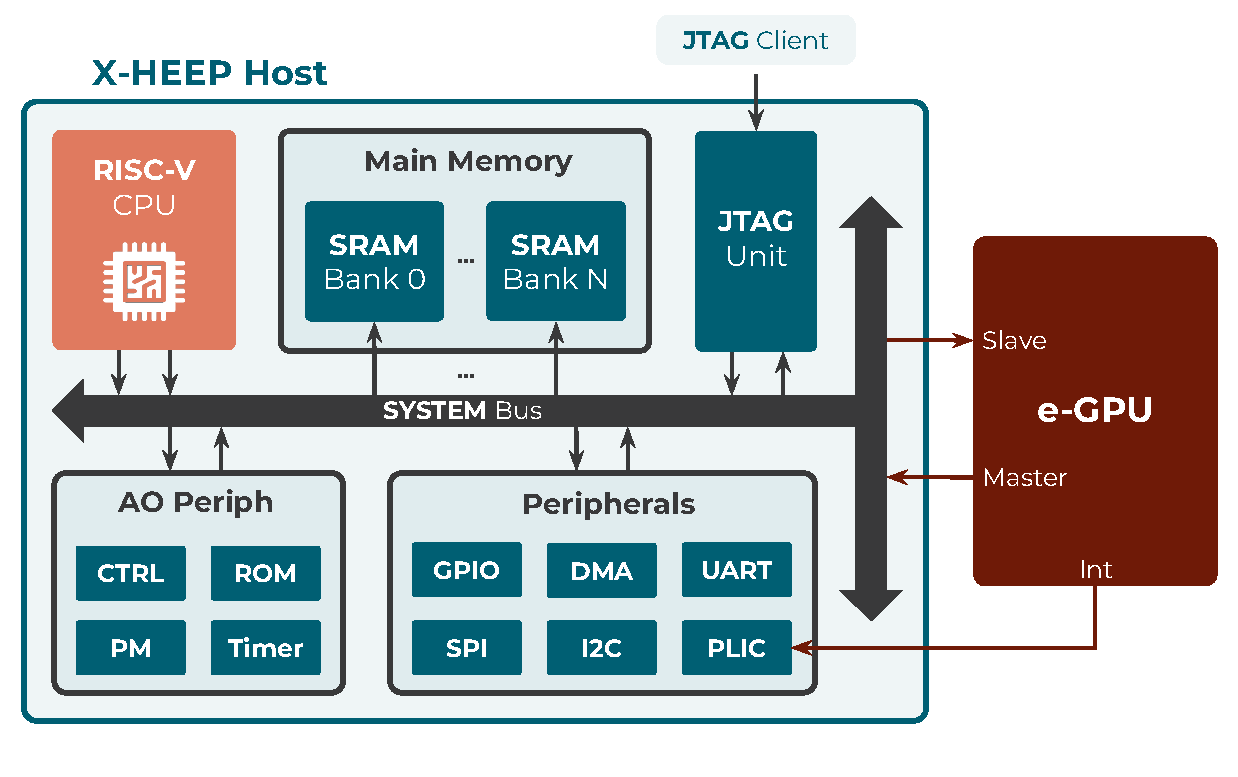
\includegraphics[width=1\textwidth]{./figures_e-gpu/apu.pdf}
                \caption{Integration of the proposed \mbox{e-GPU} with the X-HEEP host~\cite{x-heep}, resulting in the complete APU system.}
                \label{fig:apu}
            \end{figure}
        
            This modular and low-overhead interface design makes the \mbox{e-GPU} suitable for integration into a wide range of TinyAI platforms, where energy constraints and software simplicity are critical design considerations.

        \subsection{Host Configuration}
        
            The \mbox{X-HEEP}~\cite{x-heep} platform is selected as the host for the proposed APU system due to its open-source nature, modular architecture, and configurability, which collectively simplify accelerator integration and enable energy-aware customization. The selected configuration leverages a balanced set of IP blocks designed to support low-power, real-time workloads while offering sufficient flexibility for system-level design exploration.
        
            Specifically, the host is configured with the following components:

            \vspace{-1em}
            \begin{itemize}
                \item \textbf{Lightweight RISC-V CPU:} A \mbox{RI5CY} core~\cite{ri5cy} is instantiated as the main processor. Optimized for control-centric tasks, this core delegates performance-critical computations to the \mbox{e-GPU}, thereby maintaining a low overall power profile.
        
                \item \textbf{Dual SRAM Banks:} Two \SI{32}{\kibi\byte} SRAM banks are configured in contiguous addressing mode. This setup supports efficient and conflict-free memory access by enabling separate memory allocation for the CPU and the accelerator, thereby improving memory bandwidth and reducing contention.
        
                \item \textbf{Fully Connected Crossbar:} The internal interconnect consists of a fully connected crossbar that ensures high-bandwidth communication between the processor, memory banks, and the e-GPU. This architecture guarantees predictable performance under concurrent access patterns, which is critical in real-time TinyAI workloads.
        
                \item \textbf{Interrupt Controller:} A flexible platform-level interrupt controller (PLIC) handles asynchronous events from both internal peripherals and external accelerators. In this use case, it is responsible for receiving kernel completion signals from the \mbox{e-GPU} and dispatching corresponding service routines on the host CPU.
        
                \item \textbf{Power manager:} The system includes a power management unit (PM) capable of controlling both internal domains and external accelerators. It manages clock gating and power gating signals, ensuring that inactive units, including the \mbox{e-GPU}, can be fully or partially shut down to reduce energy consumption.
        
                \item \textbf{Debug Unit:} A JTAG-compatible debug unit provides full system visibility and control. It allows breakpoint insertion, register inspection, and single-step execution, which are essential features during development, integration, and debugging of the host-accelerator system.
        
                \item \textbf{eXtendible Accelerator InterFace (XAIF):} The XAIF is configured to expose one OBI master port, one OBI slave port, and one interrupt interface, matching the requirements of the \mbox{e-GPU}. This enables plug-and-play integration of the accelerator, simplifying system validation and reducing software stack complexity.
            \end{itemize}
            \vspace{-1em}
        
            This host configuration provides the necessary infrastructure to support flexible and energy-efficient execution of heterogeneous workloads. It enables streamlined accelerator communication, power-aware scheduling, and straightforward integration of the proposed \mbox{e-GPU} into TinyAI applications.

        \subsection{Tiny-OpenCL Runtime}
        
            Standard OpenCL implementations such as \mbox{PoCL}~\cite{pocl} are designed to operate on systems with full-fledged operating systems like Linux, which provide essential services including file systems, dynamic linking, and multi-threading. These runtime environments typically manage kernel compilation, buffer allocation, and accelerator control from the host side. However, in the context of the proposed APU, the host system is a lightweight microcontroller, \mbox{X-HEEP}, which lacks the ISA support and system resources required to run such traditional operating systems.
        
            Instead, the \mbox{X-HEEP} platform relies on \emph{Newlib}~\cite{newlib}, a lightweight and open-source C standard library tailored for embedded systems. \mbox{Newlib} provides basic C library functions for I/O, memory management, and string operations, but does not support features like file systems and multi-threading. As a result, the host application must be statically compiled into a single binary, and all library dependencies must be resolved at compile time since no dynamic linking is supported. Furthermore, the lack of multi-threading support mandates that the application execute in a single thread.
        
            To support OpenCL execution in this constrained environment, the \mbox{Tiny-OpenCL} framework introduced in Section~\ref{sec:e-gpu_software} is extended with a lightweight runtime specifically designed for \mbox{Newlib}-based hosts. This runtime is compiled with the standard GNU RISC-V toolchain and implements a subset of the standard OpenCL API, adapted to operate in a bare-metal environment.
        
            The \mbox{Tiny-OpenCL} runtime provides a collection of functions that allow the host to perform the following tasks:
            
            \vspace{-1em}
            \begin{itemize}
                \item Initialize memory buffers and configure memory-mapped regions for communication with the \mbox{e-GPU}. 
                
                \item Set up kernel arguments by writing them into a reserved memory space accessible by the accelerator.
                
                \item Launch kernel execution by writing to the control registers of the \mbox{e-GPU}.
                
                \item Synchronize with the accelerator by monitoring the interrupt line or polling status registers to detect completion.
            \end{itemize}
            \vspace{-1em}
            
            By preserving the OpenCL programming model, this design enables efficient deployment of embedded applications in highly constrained environments. The resulting runtime remains lightweight and portable, providing robust support for heterogeneous execution on the proposed APU platform without relying on an operating system. Its minimal resource footprint and modular structure make it particularly suitable for real-time or battery-powered TinyAI scenarios.

    \section{Experimental Setup}
    \label{sec:experimental_setup}
    
        This section outlines the experimental campaign designed to assess the proposed \mbox{e-GPU} architecture in the context of TinyAI systems. Its goal is to explore key system-level dimensions, including area, power, performance, and energy efficiency, under varying degrees of parallelism and representative workloads. Both synthetic and application-driven scenarios are considered to investigate how architectural configurability influences system behavior and resource trade-offs.
        
        The exploration is structured around four complementary experimental components:
        
        \vspace{-1em}
        \begin{itemize}
            \item \textbf{Static characterization}: This phase investigates the hardware footprint of different \mbox{e-GPU} configurations, focusing on total silicon area and leakage power. The analysis aims to quantify the integration cost of the accelerator relative to a baseline host-only system and to study how key architectural components, such as compute units and multi-bank caches, scale with increased thread-level parallelism.
            
            \item \textbf{Overhead characterization}: This phase targets the non-computational components of kernel execution, including data transfer from host memory and runtime scheduling latency introduced by the \mbox{Tiny-OpenCL} framework. By examining these overheads across a range of matrix sizes and configurations, the analysis seeks to understand the impact of memory and scheduling activities on execution efficiency.
            
            \item \textbf{TinyBio benchmark characterization}: This phase focuses on the runtime behavior of the \mbox{e-GPU} when executing the \emph{TinyBio} benchmark suite, which comprises a set of heterogeneous kernels extracted from the MBio-Tracker application~\cite{mbio_tracker}. Each pipeline stage, pre-processing, delineation, feature extraction, and prediction, is characterized individually to evaluate how well the architecture accommodates diverse computational and control patterns.
            
            \item \textbf{Trade-off discussion}: The final phase synthesizes the insights gathered from the previous analyses to identify optimal trade-offs between performance, energy, and hardware cost. The comparison between the baseline host and the various \mbox{e-GPU} configurations is used to guide the selection of appropriate architectural parameters for different TinyAI deployment scenarios.
        \end{itemize}
        \vspace{-1em}
        
        The remainder of this section details the setup used to conduct these experiments. First, the selected \mbox{e-GPU} configurations are introduced, including compute unit structure, thread parallelism, and memory hierarchy. Then, the benchmark workloads are described, comprising both the synthetic matrix multiplication kernel and the representative TinyBio application. Finally, the methodology for performance, power, and energy estimation is outlined.

           \begin{table}[tp]
                \caption{Selected \mbox{e-GPU} configurations for our experiments. CU: Compute Unit.}
                \label{tbl:config}
                \centering
                \resizebox{0.6\textwidth}{!}{
                \begin{tabular}{|l|c|c|c|}
                \toprule
                \textbf{Metric} & \textbf{e-GPU 4T} & \textbf{e-GPU 8T} & \textbf{e-GPU 16T} \\
                \midrule
                Compute Units   & \multicolumn{3}{c|}{2} \\
                \midrule
                Parall. Threads & 2 xCU & 4 xCU & 8 xCU \\
                \midrule
                Concur. Warps   & \multicolumn{3}{c|}{4 xCU} \\
                \midrule
                I-Cache Size    & \multicolumn{3}{c|}{\SI{2}{\kibi\byte} xCU} \\
                \midrule
                I-Cache Banks   & \multicolumn{3}{c|}{1 xCU} \\
                \midrule
                I-Cache Line    & \multicolumn{3}{c|}{\SI{16}{\byte} xCU} \\
                \midrule
                D-Cache Size    & \multicolumn{3}{c|}{\SI{16}{\kibi\byte}} \\
                \midrule
                D-Cache Banks   & 2 & 4 & 8 \\
                \midrule
                D-Cache Line    & \SI{8}{\byte} & \SI{16}{\byte} & \SI{32}{\byte} \\
                \bottomrule
                \end{tabular}
                }
            \end{table}

        \subsection{e-GPU Configurations}
        
            The selected configurations for the experimental evaluation are summarized in Table~\ref{tbl:config}. Each instance is equipped with two compute units, while the number of parallel threads per unit varies from two to eight. This range captures different trade-offs between performance and resource usage, enabling an exploration of how parallelism scales under constrained area and power budgets typical of TinyAI scenarios.
        
            To mitigate memory access latency and maintain high throughput, each compute unit supports four concurrent warps. Given that the shared data cache has a read latency of four cycles, this configuration ensures that the pipeline can be saturated with four outstanding memory requests, effectively achieving a sustained throughput of one access per cycle under ideal conditions.
        
            Each compute unit integrates a private instruction cache configured with a single memory bank. This choice simplifies the cache control logic, reducing both area and dynamic power consumption. A line size of \SI{16}{\byte}, equivalent to four RISC-V instructions, enhances spatial locality and supports instruction prefetching. The total instruction cache capacity is \SI{4}{\kibi\byte}, evenly partitioned between the two compute units, ensuring that all kernels in the benchmark suite fit entirely in cache, thus avoiding instruction cache failures.

            \begin{table}[tp]
                \caption{Summary of benchmark workloads used to evaluate the \mbox{e-GPU} architecture.}
                \label{tbl:benchmarks}
                \centering
                \resizebox{0.85\textwidth}{!}{
                \begin{tabular}{|l|l|l|l|l|}
                    \toprule
                    \bf Benchmark & \bf Type & \bf Purpose & \bf Stages & \bf Algorithm \\
                    \midrule
                    GeMM & Synthetic & Overhead analysis & - & Mat mul \\
                    \midrule
                    MBio-Tracker & Real-world & TinyBio analysis & 
                    \begin{tabular}[c]{@{}l@{}}1. Pre-processing\\2. Delineation\\3. Feat. Extraction\\4. Prediction\end{tabular} 
                    & 
                    \begin{tabular}[c]{@{}l@{}}
                    FIR\\ 
                    Max-Min\\
                    FFT\\ 
                    SVM
                    \end{tabular} \\
                    \bottomrule
                \end{tabular}
                }
            \end{table}
        
            The shared data cache adopts a multi-bank architecture with line-interleaved addressing to maximize throughput when multiple compute units access memory simultaneously. Specifically, two cache banks are provisioned, one per compute unit, to enable parallel servicing of requests. The cache line size is defined as $T \times \SI{4}{\byte}$, where $T$ is the number of threads per compute unit. This configuration allows each thread to access one 32-bit word in a single line fetch, which is optimal for workloads with sequential access patterns.
        
            To minimize off-chip memory accesses and improve energy efficiency, the data cache is sized at \SI{16}{\kibi\byte}, which is sufficient to hold the working set of the evaluated kernels. By provisioning this level of storage and optimizing the cache geometry, the design reduces the need for frequent data transfers to and from the host main memory, further contributing to the low-power objectives of the \mbox{e-GPU}.

        \subsection{Benchmarks} 
        \label{sec:kernels}
            
            The experimental evaluation of the proposed \mbox{e-GPU} architecture is based on two complementary benchmarks: a synthetic matrix multiplication workload (GeMM) and a representative TinyBio application. Each is designed to target a specific evaluation phase, enabling both controlled measurements and realistic scenario testing. Table~\ref{tbl:benchmarks} summarizes their main characteristics, with details provided below:

            \begin{itemize}
                \item \textbf{GeMM benchmark}: It is used in the \textit{overhead characterization} phase and consists of standard matrix multiplication kernels with input dimensions ranging from $32 \times 32$ to $256 \times 256$. This workload provides a robust baseline for evaluating raw computational throughput and memory bandwidth utilization. Its regular structure allows for controlled variation of arithmetic intensity and data movement patterns, making it particularly suitable for isolating and analyzing runtime overheads such as data transfers and kernel scheduling.
                
                \item \textbf{MBio-Tracker benchmark}: It is used in the \textit{TinyBio benchmark characterization} phase and includes a set of real-world kernels drawn from the \textit{MBio-Tracker} application~\cite{mbio_tracker}, a physiological signal processing pipeline designed to assess cognitive workload using data collected from wearable sensors. This application exemplifies practical TinyAI use cases in digital health, ambient intelligence, and low-power behavioral monitoring.

                The MBio-Tracker pipeline comprises four heterogeneous stages, each with distinct computational and memory access profiles:
        
                \begin{enumerate}[label=(\alph*)]
                    \item \textbf{Pre-processing}: It applies a FIR filter to the raw biosignal to eliminate high-frequency noise and motion artifacts. This stage improves signal quality and prepares the data for subsequent analysis by enforcing consistent amplitude and frequency characteristics.
                
                    \item \textbf{Delineation}: It identifies local extrema (peaks and troughs) in the filtered signal to detect key physiological events, such as breathing cycles or heartbeats. This process involves control-flow-heavy logic and conditional branching, making it representative of non-uniform, event-driven workloads.
                
                    \item \textbf{Feature extraction}: It computes a range of statistical and spectral features from the delineated signal. Time-domain metrics include mean, median, and root mean square (RMS), while spectral features are obtained using the Stockham FFT, which enables efficient frequency analysis through a regular, stage-wise computation pattern.
                
                    \item \textbf{Prediction}: It uses a linear support vector machine (SVM) classifier to infer the cognitive workload of the subject from the extracted features. The classification phase is dominated by vector operations and conditional comparisons, and it reflects the decision-making stage common in many TinyAI inference tasks.
                \end{enumerate}
        
                These kernels are selected for their algorithmic diversity, including regular compute-bound stages (e.g., FIR and FFT) as well as control- and memory-intensive operations (e.g., delineation and classification). This combination provides a comprehensive basis for evaluating the adaptability, scalability, and efficiency of the \mbox{e-GPU} across a wide range of TinyAI workload characteristics.
            \end{itemize}

        \subsection{Methodology}
        
            To evaluate area, power, and energy, each complete APU system is synthesized using TSMC \SI{16}{\nano\meter} CMOS technology, operating at \SI{0.8}{\volt} and \SI{300}{\mega\hertz}. Logic synthesis is performed using Synopsys Design Compiler, and memory blocks are instantiated with foundry-provided SRAM macros. Post-synthesis timing simulations are executed on representative workloads to capture switching activity, and Value Change Dump (VCD) files are generated. These VCD traces are then analyzed using Synopsys PrimePower to estimate both dynamic and leakage energy consumption.

    \section{Experimental Results}
    \label{sec:experimental_results}

        This section presents the results of the experimental campaign introduced in Section~\ref{sec:experimental_setup}, evaluating the proposed \mbox{e-GPU} architecture across multiple system configurations and workloads. Its goal is to assess the performance, energy efficiency, and hardware overheads of the platform under realistic operating conditions representative of TinyAI scenarios. The analysis is structured according to the four presented experimental components: \textit{Static Characterization}, \textit{Overhead Characterization}, \textit{TinyBio Benchmark Characterization}, and \textit{Trade-off Discussion}. Each subsection focuses on a specific aspect of the system behavior and collectively supports a comprehensive evaluation of the proposed \mbox{e-GPU} solution.

        \subsection{Static Characterization}
        
            Table~\ref{tbl:area_leakage} and Figure~\ref{fig:area_leakage} present the post-synthesis breakdown of area and leakage power across the evaluated systems. The complete APU systems occupy a total area ranging from \SI{0.24}{\milli\meter\squared} to \SI{0.38}{\milli\meter\squared}, depending on the selected \mbox{e-GPU} configuration. These results confirm the feasibility of deploying the proposed design in TinyAI use cases, where the total SoC footprint is often constrained to a few square millimeters. Despite integrating two compute units and a shared cache hierarchy, the \mbox{e-GPU} remains compact and efficient. Compared to the baseline host-only system, which occupies \SI{0.15}{\milli\meter\squared}, the \mbox{e-GPU} introduces a modest area overhead of \SI{1.6}{\times} to \SI{2.5}{\times}, which is justified by the performance improvements of \SI{3.6}{\times} to \SI{15.1}{\times}, as shown in Figure~\ref{fig:proc_energy}.
        
            The breakdown of area contributions reveals clear scaling behavior across components. The instruction cache, implemented as a fixed-capacity single-bank structure, remains constant across all configurations. This behavior is expected, as the instruction cache is not duplicated or scaled when the number of threads increases. It is designed to accommodate all kernel binaries used in the experiments, which are modest in size due to the limited computational complexity of TinyAI workloads.
        
            In contrast, the data cache area increases slightly in different configurations, although the total data storage capacity is maintained constant at \SI{16}{\kibi\byte}. This increase is due to architectural enhancements introduced to support higher degrees of parallelism. In particular, the cache must accommodate more simultaneous read/write requests, requiring additional access ports and wider cache lines. To implement wider lines efficiently, the cache is banked: two banks for four-thread configurations, four for eight-thread configurations, and eight for 16-thread configurations. This approach improves bandwidth and allows multiple threads to access memory concurrently with minimal contention. However, it also introduces overhead in terms of interconnect complexity, control logic, and physical separation between banks, all contributing to the observed area growth.
        
            The most significant contributor to the total area is the compute unit. As the number of threads per compute unit increases from two to eight, the compute logic must scale accordingly. This scaling includes the instantiation of additional arithmetic pipelines, an expanded register file to accommodate private thread data, and enhanced control and scheduling logic to manage concurrent warp execution. These additions are critical to ensure full hardware utilization and high throughput in highly parallel workloads. The compute unit area nearly doubles across configurations, reflecting the cost of the additional resources used to support the higher parallelism.

            \begin{table}[tp]
                \caption{Area and leakage breakdown across accelerator configurations with percentage contribution to total.}
                \label{tbl:area_leakage}
                \centering
                \resizebox{1\textwidth}{!}{
                \begin{tabular}{|l|c c c c|c c c c|c c c c|}
                    \toprule
                    \multirow{3}{*}{\bf Module} 
                    & \multicolumn{4}{c|}{\bf e-GPU 4T} 
                    & \multicolumn{4}{c|}{\bf e-GPU 8T} 
                    & \multicolumn{4}{c|}{\bf e-GPU 16T} \\
                    
                    & \bf Area & & \bf Lkg &
                    & \bf Area & & \bf Lkg &
                    & \bf Area & & \bf Lkg & \\
                    
                    & [mm$^2$] & \% & [$\mu$W] & \%
                    & [mm$^2$] & \% & [$\mu$W] & \% 
                    & [mm$^2$] & \% & [$\mu$W] & \% \\
                    
                    \midrule           
                    Host                  & 0.1477   & 61.27    & 29.50     & 22.67 
                                          & 0.1477   & 50.59    & 29.50     & 15.30
                                          & 0.1477   & 38.57    & 29.50     & 9.66 \\
                    Instr. Caches         & 0.0161   & 6.68     & 15.00     & 11.53 
                                          & 0.0161   & 5.50     & 15.03     & 7.79 
                                          & 0.0161   & 4.19     & 15.00     & 4.91 \\
                    Data Cache            & 0.0275   & 11.41    & 20.83     & 16.01 
                                          & 0.0353   & 12.10    & 28.90     & 14.99 
                                          & 0.0454   & 11.86    & 40.10     & 13.13 \\
                    Compute Units         & 0.0484   & 20.08    & 63.12     & 48.51 
                                          & 0.0911   & 31.21    & 117.30    & 60.82 
                                          & 0.1714   & 44.77    & 218.00    & 71.39 \\
                    Mem. Interface        & 0.0011   & 0.44     & 1.32      & 1.02 
                                          & 0.0015   & 0.51     & 1.79      & 0.93  
                                          & 0.0020   & 0.53     & 2.42      & 0.79  \\
                    Controller            & 0.0003   & 0.12     & 0.33      & 0.26  
                                          & 0.0003   & 0.10     & 0.33      & 0.17  
                                          & 0.0003   & 0.07     & 0.33      & 0.11  \\
                    \midrule
                        \bf APU Total     & \textbf{0.24}     & \textbf{100}      & \textbf{130.10}    & \textbf{100} 
                                          & \textbf{0.29}     & \textbf{100}      & \textbf{192.85}    & \textbf{100} 
                                          & \textbf{0.38}     & \textbf{100}      & \textbf{305.35}    & \textbf{100} \\
                    \bottomrule
                \end{tabular}
                }
            \end{table}
        
            A similar scaling trend is observed in the static power domain. As shown in Figure~\ref{fig:area_leakage}, the leakage power of the APU systems increases from \SI{130.13}{\micro\watt} to \SI{305.32}{\micro\watt}. This represents an overhead of \SI{4.4}{\times} to \SI{10.3}{\times} compared to the host, which dissipates \SI{29.50}{\micro\watt}. Notably, this growth remains bounded within the sub-milliwatt range, making the platform well-suited for power-constrained TinyAI systems.
        
            Overall, these results highlight the scalability and design flexibility of the proposed architecture. Thanks to its modular design, the compute units and cache subsystems can be configured independently, allowing the system to be tailored to application-specific constraints and performance targets. Most of the observed increases in area and leakage power are attributed to the compute logic, which scales proportionally with the number of threads and arithmetic pipelines. In contrast, both the instruction and data caches maintain a compact footprint and stable power profile, even as parallelism increases. This architectural balance enables designers to scale up parallelism to meet workload demands while avoiding disproportionate penalties in overall silicon area or static power consumption.

        \subsection{Overhead Characterization}

            \begin{figure}[t]
                \centering
                
\includegraphics[width=0.98\textwidth]{./figures_e-gpu/area_leakage.pdf}
                \caption{Breakdown of area and leakage power for the selected e-GPU systems compared to the baseline host system.}
                \label{fig:area_leakage}
            \end{figure}

            Table~\ref{tbl:overheads} and Figure~\ref{fig:overheads} provide a detailed breakdown of the system-level overheads relative to kernel computation time for matrix multiplication kernels of increasing size, executed on the selected \mbox{e-GPU} configurations. Two main overhead components are analyzed: \emph{transferring} and \emph{scheduling}. These represent the non-computational phases of execution that must be accounted for when evaluating total acceleration latency and energy consumption.

            \subsubsection*{Transferring overhead} 
            
                This overhead captures the time required to preload the kernel input and output data from the host main memory into the shared data cache of the \mbox{e-GPU}. This transfer phase takes place before the kernel execution and is performed using the memory interface described in Section~\ref{sec:apu_system}. The interface supports a bandwidth of \SI{32}{\bit\per\cycle}, which is typical of low-power platforms. Assuming that the data cache is provisioned with sufficient capacity to accommodate the kernel working set, the transferred data remains resident throughout all subsequent kernel executions. This minimizes repeated data movement, improving both performance and energy efficiency by reducing off-chip accesses.
        
                As expected, the absolute transfer time scales with problem size, increasing from approximately \SI{27}{\micro\second} for a $32\times32$ matrix to around \SI{1.7}{\milli\second} for a $256\times256$ matrix in the most parallel configuration. However, a key observation is that, at fixed problem size, increasing the number of threads per compute unit leads to a modest reduction in transfer time. This effect is attributed to the adoption of wider cache lines in higher-performance configurations. Wider lines increase the effective granularity of memory requests, allowing more data to be prefetched with each miss and thereby improving memory subsystem efficiency. This also enhances the potential overlap between data transfers and computation, particularly in deeper cache pipelines, contributing to better overall utilization of available bandwidth.

                \begin{table}[tp]
                    \caption{Cycle breakdown by matrix size and execution phase across configurations.}
                    \label{tbl:overheads}
                    \centering
                    \resizebox{0.9\textwidth}{!}{
                    \begin{tabular}{|c|c|c c|c c|c c|}
                        \hline
                        \bf Matrix Size & \bf Phase 
                        & \multicolumn{2}{c|}{\bf e-GPU 4T} 
                        & \multicolumn{2}{c|}{\bf e-GPU 8T} 
                        & \multicolumn{2}{c|}{\bf e-GPU 16T} \\
                        &  
                        & \bf Time [cc] & \% 
                        & \bf Time [cc] & \% 
                        & \bf Time [cc] & \% \\
                        \hline
                        \multirow{3}{*}{$32\times32$}
                        & Transferring & 18068 & 20 & 11416 & 20 & 8088  & 20 \\
                        & Scheduling   & 13776 & 15 & 9204  & 15 & 7096  & 17 \\
                        & Computing    & 58716 & 65 & 38962 & 65 & 25788 & 63 \\
                        \hline
                        \multirow{3}{*}{$64\times64$}
                        & Transferring & 72272  & 23 & 45664  & 22 & 32352  & 23 \\
                        & Scheduling   & 13776  &  4 & 9204   &  4 & 7096   &  5 \\
                        & Computing    & 234864 & 73 & 155848 & 74 & 103152 & 72 \\
                        \hline
                        \multirow{3}{*}{$128\times128$}
                        & Transferring & 289088 & 23 & 182656 & 23 & 129408 & 24 \\
                        & Scheduling   & 13776  &  1 & 9204   &  1 & 7096   &  1 \\
                        & Computing    & 939456 & 76 & 623392 & 76 & 412608 & 75 \\
                        \hline
                        \multirow{3}{*}{$256\times256$}
                        & Transferring & 1156352 & 24 & 730624  & 23 & 517632  & 24 \\
                        & Scheduling   & 13776   &  \textasciitilde 0 & 9204    &  \textasciitilde 0 & 7096    &  \textasciitilde 0 \\
                        & Computing    & 3757824 & 76 & 2493568 & 77 & 1650432 & 76 \\
                        \hline
                    \end{tabular}
                    }
                \end{table}

                Importantly, despite the growing transfer latency for larger problem sizes, the relative impact of data movement stabilizes at slightly above \SI{20}{\percent} of the total execution time. This implies that the performance benefits of increased parallelism compensate for the additional cost of transferring larger input matrices. The result confirms that the platform maintains a balanced data-compute ratio across workloads, an essential property for energy-efficient execution in memory-bound applications.

            \vspace{-1em}
            \subsubsection*{Scheduling overhead}
            
                On the other hand, this overhead corresponds to the time taken by the \mbox{Tiny-OpenCL} scheduling functions, as described in Section~\ref{sec:e-gpu_software}, to allocate computing resources and assign work items to active threads. Since the framework supports dynamic scheduling at execution time, this overhead depends on both the total number of work items and the granularity of the hardware configuration.
        
                In our experiments, the total number of work items matches the hardware capacity, which isrk-items matches the hardware capacity, that is, the number of compute units multiplied by the number of threads per unit and the number of concurrent warps. This setup ensures a one-to-one mapping between work items and execution contexts, thereby avoiding unnecessary iterations and simplifying the scheduling logic.
        
                As a result, scheduling time remains constant at approximately \SI{25}{\micro\second}, regardless of matrix size or system configuration. Although this time may seem negligible in absolute terms, its relative contribution to the total execution time is more significant for smaller problems. Specifically, scheduling overhead accounts for roughly \SI{15}{\percent} of total latency for the smallest kernels and drops below \SI{1}{\percent} for the largest ones. This diminishing trend highlights the scalability of the \mbox{Tiny-OpenCL} framework, which introduces minimal scheduling overhead while offering fine-grained control and adaptability to different execution configurations.
                
                \begin{figure}[t]
                    \centering
                    
\includegraphics[width=0.98\textwidth]{./figures_e-gpu/overheads.pdf}
                    \caption{Breakdown of execution time (in logarithmic scale) and normalized execution time for the selected e-GPU systems across matrix multiplication kernels.}
                    \label{fig:overheads}
                \end{figure}
        
            In summary, the overhead analysis demonstrates that both the transferring and scheduling components remain bounded and predictable, even as the problem sizes and parallelism increase. The transferring phase is efficiently amortized through the reuse of input data across multiple kernel stages, while the scheduling logic exhibits excellent scalability, becoming negligible for problem sizes equal to or larger than a $256 \times 256$ matrix or equivalent. These findings reinforce the viability of the proposed \mbox{e-GPU} architecture and the \mbox{Tiny-OpenCL} framework as a low-overhead solution for energy-efficient acceleration in TinyAI systems.

            \begin{table}[tp]
                \caption{Processing time, power, and normalized performance metrics across processing elements for representative processing phases.}
                \label{tbl:proc_energy}
                \centering
                \resizebox{1\textwidth}{!}{
                \begin{tabular}{|l|c|c|c|c|c|}
                \toprule
                \bf Phase & \bf Proc. Element & \bf Proc. Time [cc] & \bf Speedup [\si{\times}] & \bf Power [\si{\milli\watt}] & \bf Energy Red. [\si{\times}] \\
                \midrule
                Pre-processing     & CPU  & 91379  & -     & 5.7   & -    \\
                                   & 4T   & 25736  & 3.6   & 12.0   & 1.7  \\
                                   & 8T   & 12260  & 7.5   & 20.0   & 2.1  \\
                                   & 16T  & 6042   & 15.1  & 28.0   & 3.1  \\
                \midrule
                Delineation        & CPU  & 19841  & -     & 5.7  & -    \\
                                   & 4T   & 6434   & 3.1   & 12.0  & 1.5  \\
                                   & 8T   & 3065   & 6.5   & 20.0  & 1.8  \\
                                   & 16T  & 1511   & 13.1  & 28.0  & 2.7  \\
                \midrule
                Feature Extraction & CPU  & 173955 & -     & 5.7  & -    \\
                                   & 4T   & 52759  & 3.3   & 12.0  & 1.6  \\
                                   & 8T   & 25133  & 6.9   & 20.0  & 2.0  \\
                                   & 16T  & 12386  & 14.0  & 28.0  & 2.9 \\
                \midrule
                Overall            & CPU  & 95058  & -     & 5.7  & -    \\
                                   & 4T   & 28310  & 3.4   & 12.0  & 1.6  \\
                                   & 8T   & 13486  & 7.0   & 20.0  & 2.0 \\
                                   & 16T  & 6646   & 14.3  & 28.0  & 2.9 \\
                \bottomrule
                \end{tabular}
                }
            \end{table}
        
        \subsection{TinyBio Benchmark Characterization}
        
            Table~\ref{tbl:proc_energy} and Figure~\ref{fig:proc_energy} present the performance and energy efficiency gains achieved by the proposed APU systems when executing the TinyBio benchmark introduced in Section~\ref{sec:experimental_setup}. The metrics are expressed as speed-up and energy reduction relative to the baseline host-only configuration. Each stage of the TinyBio processing pipeline is individually analyzed to highlight the interaction between algorithmic characteristics and architectural features.

            \vspace{-1em}
            \subsubsection*{Pre-processing} 
            
                The first stage of the pipeline applies a FIR filter to the raw input data. This algorithm is inherently data-parallel: each output sample can be computed independently from its neighbors, allowing concurrent execution across multiple threads. The filter relies on a fixed number of multiply-accumulate (MAC) operations per output, which map efficiently to the arithmetic units within each compute unit of the \mbox{e-GPU}. Additionally, memory accesses follow a regular, sequential pattern, enabling optimal cache usage and coalesced accesses in the data cache. These characteristics lead to high computational efficiency and excellent resource utilization. As a result, speed-up ranges from \SI{3.6}{\times} to \SI{15.1}{\times} depending on the hardware configuration, with a corresponding energy reduction of \SI{1.7}{\times} to \SI{3.1}{\times}.

            \vspace{-1em}
            \subsubsection*{Delineation} 
            
                The second stage performs control-intensive signal analysis to detect peaks and troughs. Unlike the FIR filter, this workload involves a mix of serial and parallel operations, along with conditional logic to detect turning points in the signal. These branches introduce divergence between threads, which reduces parallel efficiency as divergent paths must be serialized using warp masking. As GPUs are optimized for throughput rather than low-latency conditional execution, this class of workload is inherently less suited to SIMT architectures. Nevertheless, due to the alternation of serial and parallel operations, the \mbox{e-GPU} still achieves speed-ups ranging from \SI{3.1}{\times} to \SI{13.1}{\times}, with corresponding energy reductions of \SI{1.5}{\times} to \SI{2.7}{\times}. These results demonstrate that even control-bound workloads can benefit significantly from architectural efficiency.

                \begin{figure}[t]
                    \centering
                    
\includegraphics[width=0.98\textwidth]{./figures_e-gpu/proc_energy.pdf}
                    \caption{Speed-up and energy reduction of the TinyBio benchmark on the selected e-GPU systems compared to the baseline host system.}
                    \label{fig:proc_energy}
                \end{figure}

            \vspace{-1em}
            \subsubsection*{Feature Extraction \& Prediction} 
            
                The third stage computes both time-domain and frequency-domain features. Among the latter, the Stockham FFT is used due to its regular structure and ability to avoid explicit bit-reversal permutations. Unlike Cooley–Tukey, the Stockham variant uses ping-pong buffers and computes butterfly operations in a stage-wise fashion, where each stage processes all data points using a regular pattern of accesses. These properties favor cache locality and allow parallel execution of butterfly pairs within each stage. However, synchronization is required between stages, limiting inter-stage parallelism. Despite this constraint, the e-GPU systems achieve performance improvements ranging from \SI{3.3}{\times} to \SI{14.0}{\times}, while consuming \SI{1.6}{\times} to \SI{2.9}{\times} less energy than the baseline CPU execution.

                In the final stage, an SVM classifier predicts the cognitive workload based on the extracted features. This computation primarily involves vector dot products and comparison operations and exhibits limited computational intensity and memory access. As its execution time and energy consumption are negligible compared to the other stages, the prediction step is aggregated with the feature extraction stage for clarity.

            \vspace{-1em}
            \subsubsection*{Overall Performance} 
            
                When considering the full processing pipeline of MBio-Tracker, the \mbox{e-GPU} achieves consistent and significant improvements across all stages. Aggregated over the entire benchmark, the system delivers speed-ups of \SI{3.4}{\times} to \SI{14.3}{\times}, with energy savings of \SI{1.6}{\times} to \SI{2.9}{\times}, depending on the degree of parallelism and system configuration.
        
                These results validate the suitability of the proposed \mbox{e-GPU} platform for real-world TinyAI workloads. Moreover, they demonstrate how the co-design of hardware and software in the \mbox{Tiny-OpenCL} framework enables efficient utilization of both parallelism and memory locality, even under stringent area and power constraints.

        \subsection{Trade-off Discussion}
        
            The experimental results underscore the architectural trade-offs and design considerations involved in deploying efficient compute platforms for TinyAI applications. Each evaluated system, ranging from the standalone host to the increasingly capable \mbox{e-GPU} configurations, represents a different point in the design space between complexity, performance, and energy efficiency.
        
            The baseline host system is optimized for simplicity and minimal resource usage. It offers the smallest area and leakage power footprint among all configurations, making it particularly suitable for extremely constrained edge scenarios such as single-sensor wearables or implantable devices. Its architecture, centered on a lightweight RISC-V CPU, ensures that system-level control and simple tasks can be executed with minimal energy overhead. However, the host CPU quickly reaches its performance limits when tasked with more demanding TinyAI kernels, especially those involving high data throughput, signal processing, or machine learning inference. In such scenarios, prolonged execution times directly increase dynamic energy consumption, negating the initial benefits of low leakage and small footprint.
        
            In contrast, the APU systems introduce moderate increases in area from \SI{0.24}{\milli\meter\squared} to \SI{0.38}{\milli\meter\squared}, but offer substantially improved performance and energy efficiency. The architectural design leverages configurable parallelism through compute units, threads, and warps, and a unified memory hierarchy that eliminates explicit data transfers. As shown in the benchmark analysis, this results in speed-ups of \SI{3.1}{\times} to \SI{15.1}{\times} and energy reductions of \SI{1.5}{\times} to \SI{3.1}{\times}, depending on the specific workload characteristics and system configuration.
        
            These benefits are particularly pronounced in data-parallel workloads with regular memory access patterns, such as FIR filters or FFTs. In these cases, the \mbox{e-GPU} architecture exhibits high efficiency due to its ability to maximize instruction throughput and memory bandwidth utilization. Even in more control-dominated workloads like signal delineation, where warp divergence becomes a limiting factor, the system maintains competitive performance and energy benefits. This resilience highlights the strength of the presented \mbox{Tiny-OpenCL} framework, which facilitates efficient scheduling and resource management even under non-ideal conditions.

    \section{Summary and Conclusions}
    \label{sec:conclusions}
    
        The increasing demand for real-time, machine-learning-driven inference in resource-constrained scenarios has accelerated the shift toward edge computing. In this paradigm, processing data locally at the edge enhances latency, privacy, and energy efficiency. However, these benefits come with significant design challenges, as workloads must operate under strict area, power, and performance constraints, necessitating the development of specialized, lightweight hardware accelerators. Among such accelerators, GPUs are particularly promising due to their capacity to exploit data-level parallelism in a wide range of application scenarios. Yet, their suitability for TinyAI applications remains underexplored.
    
        To bridge this gap, this chapter presented \mbox{e-GPU}, an open-source and configurable RISC-V GPU platform for TinyAI applications. The architecture supports extensive configurability through design-time parameters, allowing developers to finely balance performance, area, and energy consumption according to the target workload. This hardware flexibility is complemented by the \mbox{Tiny-OpenCL} framework, a lightweight and efficient OpenCL-based software stack tailored for bare-metal systems without operating system support. Together, the hardware and software co-design enables high programmability and compatibility with existing GPU software tools while remaining efficient in severely constrained environments.

        The \mbox{e-GPU} was integrated into the \mbox{X-HEEP} platform~\cite{x-heep}, a modular and extensible RISC-V host, forming a complete APU. Multiple \mbox{e-GPU} configurations were synthesized using TSMC \SI{16}{\nano\meter} CMOS technology, operating at \SI{300}{\mega\hertz} and \SI{0.8}{\volt}. The experimental campaign was organized into four complementary evaluations, each addressing a specific architectural question and revealing key insights:

        \begin{itemize}
            \item \textbf{Static characterization:} The silicon cost and leakage of integrating the \mbox{e-GPU} into a minimal RISC-V host are evaluated. The total area grows from \SI{0.24}{\milli\meter\squared} in the 4-thread configuration to \SI{0.38}{\milli\meter\squared} in the 16-thread configuration, while leakage increases from \SI{130}{\micro\watt} to \SI{305}{\micro\watt}. Most of this growth comes from compute units that expand with additional threads and pipelines, whereas instruction caches remain constant. Data cache size increases slightly with higher bank counts (2–8) to sustain bandwidth.
        
            \item \textbf{Overhead characterization:} The non-computational costs of data transfers and scheduling are analyzed using a GeMM benchmark for matrix sizes from $32 \times 32$ to $256 \times 256$. Data transfers consistently account for about \SI{20}{\percent} of execution time, with higher-parallelism designs benefiting from wider cache lines that improve burst efficiency. Scheduling latency remains fixed at \SI{25}{\micro\second}, representing \SI{15}{\percent} of runtime for small kernels but falling below \SI{1}{\percent} for problem sizes equal to or larger than a $256 \times 256$ matrix multiplication.
        
            \item \textbf{TinyBio benchmark characterization:} The MBio-Tracker benchmark~\cite{mbio_tracker}, which includes FIR filtering, control-heavy delineation, FFT-based feature extraction, and SVM prediction, is evaluated. The \mbox{e-GPU} delivers speed-ups between \SI{3.1}{\times} and \SI{15.1}{\times} with energy savings from \SI{1.5}{\times} to \SI{3.1}{\times}, while keeping power consumption below \SI{28}{\milli\watt} in the 16-thread configuration. Data-parallel stages such as FIR and FFT achieve the highest gains, while delineation still benefits despite warp divergence.
        \end{itemize}
    
        In summary, this chapter has delivered a fully open-source, configurable, and energy-efficient GPU platform, paired with a matching software stack, to enable GPU acceleration in TinyAI workloads. The \mbox{e-GPU} supports diverse architectural configurations, maintains a compact and low-leakage footprint, and demonstrates clear benefits on both synthetic and real-world workloads. These results establish a strong foundation for further exploration of GPU-based architectures in resource-constrained domains, paving the way for next-generation heterogeneous processors at the extreme edge.
